\setcounter{chapter}{-1} % Para empezar a contar en 0

\chapter{Introducción}

La mayoría de ecuaciones diferenciales han sido planteadas por campos como la física. Veamos el caso de un péndulo:

\begin{figure}[H]
    \centering
    \begin{subfigure}{0.3\textwidth}
        \centering        
        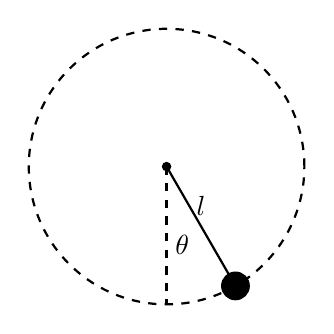
\begin{tikzpicture}
            \centering

            \def\radius{1.75}
            \def\angulo{150}

            % Desactiva los caracteres conflictivos
            \shorthandoff{>} % Para poner puntas de flecha

            \draw[thick, dashed] (0,0) circle (\radius);
            \filldraw (0,0) circle (1.5pt);
            \filldraw ({sin(\angulo)*\radius}, {cos(\angulo)*\radius}) circle (5pt);
            \draw[thick] (0,0) -- ({sin(\angulo)*\radius}, {cos(\angulo)*\radius}) node[midway, above] {$l$};
            \draw[thick, dashed] (0,0) -- (0,-\radius);
            \node at (0.2,-1) {$\theta$};

        \end{tikzpicture}

        \vspace*{0.25cm}
    \end{subfigure}
    \hfill
    \begin{subfigure}{0.6\textwidth}%
        Las condiciones que definen el péndulo son $g >0$, ya que se encuentra en la Tierra, $l$ que es la longitud del péndulo y $\theta$ que es el ángulo con respecto a la vertical.

        La ecuación que define el ángulo a lo largo del tiempo es la siguiente:
        \begin{gather*}
            \theta''(t) + \frac{g}{l} \sen(\theta(t)) = 0
        \end{gather*}
    \end{subfigure}
    \hfill
\end{figure}

Esta es una ecuación diferencial de segundo orden (ya que aparece una segunda derivada). En ella tenemos que $t$ es la variable independiente y $\theta$ es la incógnita o variable dependiente (que es una función).

Si estudiamos las soluciones de esta ecuación tenemos 
\begin{align*}
    \theta(t) &= 0, \ t\in \bb{R} \text{ es una solución (trivialmente)}\\
    \theta(t) & =\pi, \ t \in \bb{R} \text{ es también solución}\\
    \theta(t) & =2n\pi,\ \theta(t) =n\pi, \ t \in \bb{R},\ n \in \bb{Z} \text{ son infinitas soluciones}\\
\end{align*}

De esta forma podemos ver que una ecuación diferencial puede tener infinitas soluciones.

\begin{definicion}
    Podemos definir una \textbf{ecuación diferencial de primer orden} como la relación funcional dada por 
    \begin{gather*}
        \Phi (t, x(t), x'(t)) = 0
    \end{gather*}
    donde $t$ es la \textbf{variable independiente} y $x=x(t)$ es la \textbf{variable independiente} o \textbf{incógnita}.
\end{definicion}

\begin{ejemplo}
    Consideremos la ecuación diferencial dada por
    \begin{gather*}
        x(t) + x'(t)^2 = 1
    \end{gather*}
    Podemos definir\footnote{Notación física} $\Phi = \Phi(t,x,y) = x^2 + y^2 -1$, o equivalentemente\footnote{Notación moderna (matemática)}
    \begin{align*}
        \Phi : D \subset \bb{R}^3 &\rightarrow \bb{R} \\
        (t,x,y) & \mapsto \Phi(t,x,y) = x^2 + y^2 -1
    \end{align*}
    Estudiemos las soluciones a esta ecuación:

    \begin{figure}[H]
        \centering
        
        \begin{subfigure}{0.3\textwidth}
            \centering
            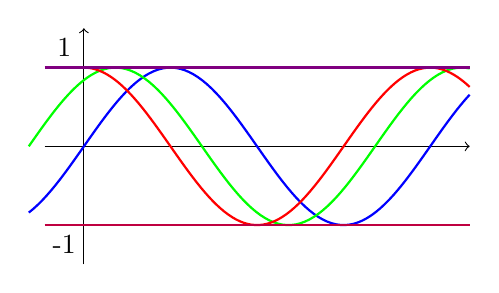
\begin{tikzpicture}
                % Desactiva los caracteres conflictivos
                \shorthandoff{>} % Para poner puntas de flecha

                \def\escalax{0.7}
                % Ejes
                \draw[->] (-0.5,0) -- (\escalax*7,0);
                \draw[->] (0,-1.5) -- (0,1.5);
            
                % Gráfica del seno
                \draw[blue, thick, domain=-1:7, samples=100] plot (\escalax*\x,{sin(\x r)});

                % Gráfica del seno trasladada
                \draw[green, thick, domain=-1:7, samples=100] plot (\escalax*\x,{sin(((\x+1) r))});
            
                % Gráfica del coseno
                \draw[red, thick, domain=0:7, samples=100] plot (\escalax*\x,{cos(\x r)});

                % Horizontales
                \draw[violet, thick] (-0.5,1) --(\escalax*7,1);
                \draw[purple, thick] (-0.5,-1) --(\escalax*7,-1);
            
                    
                % Etiquetas de los valores en el eje y
                \node at (-0.25,1.25) {1};
                \node at (-0.25,-1.25) {-1};
            \end{tikzpicture}

            \vspace*{0.5cm}
    
        \end{subfigure}
        \hfill
        \begin{subfigure}{0.6\textwidth}%
            \begin{itemize}
                \item[\textcolor{blue}{$\bullet$}] $x(t) = \sen(t)$, $t \in \bb{R}$
                \item[\textcolor{red}{$\bullet$}] $x(t)= \cos(t)$, $t \in \bb{R}$
                \item[\textcolor{violet}{$\bullet$}] $x(t)=1$, $t \in \bb{R}$
                \item[\textcolor{purple}{$\bullet$}] $x(t)=-1$, $t \in \bb{R}$
                \item[\textcolor{green}{$\bullet$}] $x(t)=\sen(t+c)$, $t \in \bb{R}$ $\forall c \in \bb{R}$ (familia uniparamétrica).
            \end{itemize}
        \end{subfigure}
        \hfill
    \end{figure}

    Podemos construir otra solución uniendo las ya dadas como por ejemplo
    \begin{gather*}
        x(t)=\left\{
        \begin{array}{ccc}
            \cos(t)& \text{ si }& t \geq 0\\
            1&  \text{ si } & t <0
        \end{array}
        \right.
    \end{gather*}
    Esta función es derivable y por tanto solución a la ecuación.

\end{ejemplo}

Típicamente estudiaremos ecuaciones diferenciales de primer orden en \textbf{forma normal}, es decir, ecuaciones que se pueden escribir como
\begin{gather*}
    x'(t) = f(t, x(t))
\end{gather*}
Esto es una subfamilia de las ecuaciones previamente descritas.

\begin{ejemplo}\ 
    \begin{enumerate}[label=\alph*)]
        \item $x'(t)=7x(t)$
        \begin{align*}
            \Phi(t,x,y)&=y-7x \\
            f(t,x) &= 7x
        \end{align*}
        Algunas de las soluciones son $x(t)=0$ (trivial), $x(t)=e^{7t}$ y $x(t)=c \cdot e^{7t},\ \ c, t\in \bb{R}$

        \item $x`(t)=7t$
        \begin{align*}
            \Phi(t,x,y)&=y-7t \\
            f(t,x) &= 7t
        \end{align*}
        Algunas de las soluciones son de la forma $x(t)=\frac{7t^2}{2} + c$, $c, t \in \bb{R}$ (realmente es una integral).
    \end{enumerate}
\end{ejemplo}

\begin{ejemplo}\
    \begin{enumerate}[label=\alph*)]
        \item $x`(t)=\sen(t)$. Sus soluciones son de la forma $x(t)=\cos(t)+c$, $c,t\in \bb{R}$
        \item $x`(t)=\sen(x(t))$. No es tan simple calcular las soluciones (aunque $x(t)=0$, $t\in \bb{R}$ es solución).
    \end{enumerate}
\end{ejemplo}

\begin{definicion}
    Una función diferencial va a venir dada por un 
    \begin{align*}
        \Phi : D \subset \bb{R}^3 &\to \bb{R}\\
        (t,x,y) &\mapsto \Phi(t,x,y) \text{ (continua)}
    \end{align*}
    donde el conjunto $D$ es un abierto de $\bb{R}^3$ conexo llamado \textbf{dominio}.

    Una \textbf{solución} de una ecuación diferencial, $\Phi(t,x(t),x`(t))=0$ será una función de la forma 
    \begin{align*}
        x: I &\to \bb{R}\\
        t & \mapsto x(t)
    \end{align*}
    donde $I$ es un intervalo abierto y $x$ tiene las siguientes propiedades:
    \begin{enumerate}
        \item[(i)] $x(t)$ es derivable en $I$.
        \item[(ii)] $(t,x(t), x'(t))\in D$\ \ \ $\forall t \in I$
        \item[(iii)] $\Phi(t, x(t), x'(t))=0$\ \ \ $\forall t \in I$
    \end{enumerate}
\end{definicion}

\begin{ejemplo}
    \begin{gather*}
        x(t)=\sqrt{2t - 38}, 
        \hspace{2cm} 
        x'(t)=\frac{1}{x(t)}
    \end{gather*}
    ¿Es $t(x)$ una solución de la ecuación dada?
    \begin{gather*}
        \Phi(t,x,y)=y - \frac{1}{x}
        \hspace{2cm} 
        D=\bb{R}\times ]0,\infty[ \times \bb{R}
        \hspace{2cm} 
        I=]19, \infty[
    \end{gather*}

    Tomamos así $D$ porque hay que quitar la discontinuidad que se produce en el plano $\{(t,x,y)\in \bb{R}^3 : x=0\}$ y además tiene que ser conexo ($\bb{R}^3$ sin un plano no es conexo).

    $I$ es el mayor intervalo abierto de $\bb{R}$ en el que $x(t)$ es derivable.

    Además, se verifica que $(t,x(t),x'(t))\in D$\ \ \ $\forall t \in I$ y 
    \begin{gather*}
        x'(t)=\frac{1}{\sqrt{2t-38}}=\frac{1}{x(t)}
    \end{gather*}
    Por lo que se verifica que es solución

\end{ejemplo}

A partir de ahora la notación que utilizaremos para expresar ecuaciones diferenciales será
\begin{gather*}
    \Phi(t,x,x') = 0 \text{ en lugar de } \Phi(x, x(t), x'(t))
\end{gather*}

\begin{ejemplo}
    \begin{align*}
        x&'=3x \hspace{1cm} (\sii x'(t)=3x(t))\\
        x(t)&=c \cdot e^{3t}
    \end{align*}

    En general, tenemos que
    \begin{align*}
        &x = \lambda x  \ \ \text{ tiene por solución }\ \  x(t)=c \cdot e ^{\lambda t}\\
        &x'=\lambda t\ \  \text{ tiene por solución }\ \  x(t)=\frac{\lambda t^2}{2} +c
    \end{align*}

\end{ejemplo}

\begin{prop}
    Dada $x(t)$ solución de $x'=\lambda x$ definida en un intervalo abierto $I$, existe $c\in \bb{R}$ de forma que $x(t)=c \cdot e^{\lambda t}$,\ \ $\forall t \in I$.

    \begin{proof}
        Sea $x(t)$ una solución. Consideramos la aplicación $e^{-\lambda t} \cdot x(t)$ que es derivable por ser producto de funciones derivables y tenemos
        \begin{gather*}
            \frac{d}{dt}\left( e^{-\lambda t} x(t)\right) = -\lambda e^{-\lambda t} x(t) + e^{-\lambda t}x`(t) \overset{(*)}{=}-\lambda e^{-\lambda t} x(t) + e^{-\lambda t}\cdot \lambda x(t) = 0
        \end{gather*}
        donde en $(*)$ he aplicado que $x'=\lambda x$ por ser solución. Al anularse la derivada de una función de clase $C^1(I)$, necesariamente tenemos que $\exists c \in \bb{R}$ tal que $e^{-\lambda t}x(t)=c$\ \ $\forall t \in I$.

        Con esta expresión, dado que la exponencial no se anula para ningún valor del dominio podemos dividir entre ella y obtenemos
        \begin{gather*}
            x(t)=c\cdot e^{\lambda t}
        \end{gather*}
    \end{proof}
\end{prop}

\section{Interpretación geométrica de una ecuación diferencial}
Sea $x'=f(x,t)$ con $f:\bb{R}^2 \to \bb{R}$, $(t,x)\mapsto f(t,x)$ una función continua. Podemos interpretar este valor $f(t,x)$ como la pendiente de una recta que pasa por $(t,x)$. A partir de esta función podemos construir los que se conoce como un \textbf{campo de direcciones} que es una regla que a cada punto del plano le asigna una dirección. Tenmos que $x'(t)=f(t,x(t))$ por lo que esta es la pendiente del campo de direcciones y por la interpretación geométrica de la derivada tenemos que este valor es la pendiente de la recta tangente en $(t,x(t))$ a la curva $x=x(t)$. Las soluciones de la ecuación diferencial son curvas que se mueven de forma tangente al campo de direcciones (se podría decir que lo "peinan").

\begin{ejemplo}\ 
    \begin{enumerate}
        \item $x'=0$. Las soluciones de esta ecuación diferencial son las de la familia uniparamétrica $x(t)=c$, $c\in \bb{R}$.
        \begin{center}
            \begin{tikzpicture}
                \draw[thick] (2,0) -- (-2,0);
                \draw[thick] (0,2) -- (0,-2);

                \def\radius{2pt}

                \def\coorx{0.5}
                \def\coory{1}
                \draw[orange, thick] (\coorx-0.3, \coory) -- (\coorx+0.3, \coory);
                \fill (\coorx, \coory) circle (\radius);

                \def\coorx{1}
                \def\coory{1.25}
                \draw[orange, thick] (\coorx-0.3, \coory) -- (\coorx+0.3, \coory);
                \fill (\coorx, \coory) circle (\radius);

                \def\coorx{0.5}
                \def\coory{-1}
                \draw[orange, thick] (\coorx-0.3, \coory) -- (\coorx+0.3, \coory);
                \fill (\coorx, \coory) circle (\radius);

                \def\coorx{-1.5}
                \def\coory{1}
                \draw[orange, thick] (\coorx-0.3, \coory) -- (\coorx+0.3, \coory);
                \fill (\coorx, \coory) circle (\radius);

                \def\coorx{-0.5}
                \def\coory{-1}
                \draw[orange, thick] (\coorx-0.3, \coory) -- (\coorx+0.3, \coory);
                \fill (\coorx, \coory) circle (\radius);

            \end{tikzpicture}
        \end{center}
        
        \item $x'=1$. Las soluciones serán de la forma $x(t)=t+c$, $t,c\in \bb{R}$. Ahora $f(t,x)=1$.
        \begin{center}
            \begin{tikzpicture}
                \draw[thick] (2,0) -- (-2,0);
                \draw[thick] (0,2) -- (0,-2);

                \def\radius{2pt}

                \def\coorx{0.5}
                \def\coory{1}
                \draw[orange, thick] (\coorx-0.2, \coory-0.2) -- (\coorx+0.2, \coory+0.2);
                \fill (\coorx, \coory) circle (\radius);

                \def\coorx{1}
                \def\coory{1.25}
                \draw[orange, thick] (\coorx-0.2, \coory-0.2) -- (\coorx+0.2, \coory+0.2);
                \fill (\coorx, \coory) circle (\radius);

                \def\coorx{0.5}
                \def\coory{-1}
                \draw[orange, thick] (\coorx-0.2, \coory-0.2) -- (\coorx+0.2, \coory+0.2);
                \fill (\coorx, \coory) circle (\radius);

                \def\coorx{-1.5}
                \def\coory{1}
                \draw[orange, thick] (\coorx-0.2, \coory-0.2) -- (\coorx+0.2, \coory+0.2);
                \fill (\coorx, \coory) circle (\radius);

                \def\coorx{-0.5}
                \def\coory{-1}
                \draw[orange, thick] (\coorx-0.2, \coory-0.2) -- (\coorx+0.2, \coory+0.2);
                \fill (\coorx, \coory) circle (\radius);

            \end{tikzpicture}
        \end{center}
        \item $x'=x$. En general, $x(t)=c e^t$, $c,t\in \bb{R}$ %TODO: hacer dibujo
        \item $x'=t^2+x^2$. Con las funciones elementales básicas no vamos a encontrar una solución, sin embargo el campo de direcciones nos permite hacernos una idea de como son estas funciones (no elementales)(No podemos definir el movimiento mediante una fórmula sino con la ley que lo describe). %TODO: hacer dibujo

        % \definecolor{qqttzz}{rgb}{0,0.2,0.6}
\definecolor{qqzzqq}{rgb}{0,0.6,0}

\begin{center}
    \resizebox{10cm}{!}{%
    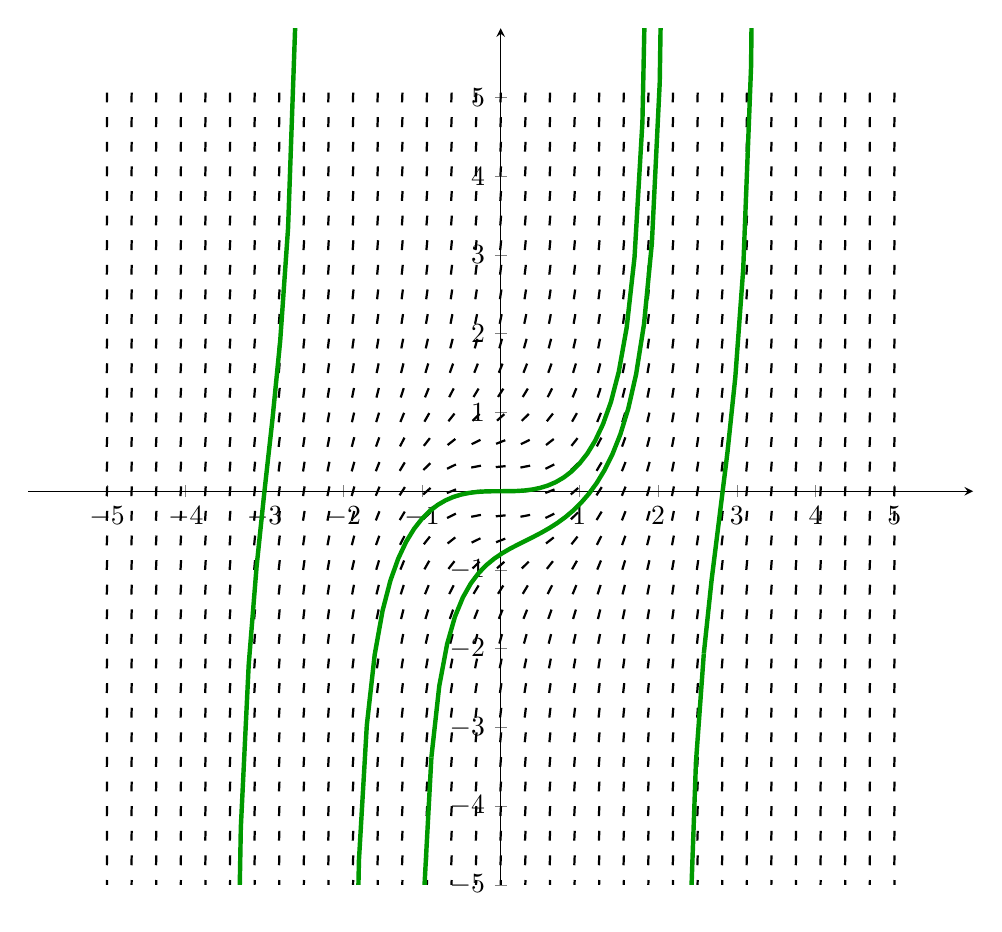
\begin{tikzpicture}%[line cap=round,line join=round,>=triangle 45,x=1cm,y=1cm]
        \begin{axis}[
        x=1cm,y=1cm,
        axis lines=middle,
        xmin=-6,
        xmax=6,
        ymin=-5,
        ymax=5.88,
        xtick={-5,-4,...,5},
        ytick={-5,-4,...,5}]
        \clip(-9.86,-10.74) rectangle (28.54,5.88);
        \draw[line width=0.8pt] (-5.001249750074975,-5.06248750374875) -- (-4.998750249925025,-4.93751249625125)(-5.001330259914028,-4.749985841664821) -- (-4.998669740085972,-4.625014158335179)(-5.001415565985464,-4.437483967327154) -- (-4.998584434014536,-4.312516032672846)(-5.001505445440851,-4.12498186644159) -- (-4.998494554559149,-4.00001813355841)(-5.001599475969558,-3.8124795300608354) -- (-4.998400524030442,-3.6875204699391646)(-5.001696986859959,-3.4999769576371733) -- (-4.998303013140041,-3.3750230423628267)(-5.001797009566536,-3.1874741607115915) -- (-4.998202990433464,-3.0625258392884085)(-5.001898233680383,-2.8749711670204317) -- (-4.998101766319617,-2.7500288329795683)(-5.001998976785761,-2.5624680245550473) -- (-4.998001023214239,-2.4375319754449527)(-5.002097179020561,-2.2499648048116354) -- (-4.997902820979439,-2.1250351951883646)(-5.002190434338555,-1.9374616041853592) -- (-4.997809565661445,-1.8125383958146408)(-5.0022760693001445,-1.6249585423184125) -- (-4.9977239306998555,-1.5000414576815875)(-5.0023512755338135,-1.3124557563669201) -- (-4.9976487244661865,-1.1875442436330799)(-5.002413293287644,-0.999953390744681) -- (-4.997586706712356,-0.875046609255319)(-5.0024596315745065,-0.6874515829464529) -- (-4.9975403684254935,-0.5625484170535471)(-5.0024882979796805,-0.3749504473415869) -- (-4.9975117020203195,-0.2500495526584131)(-5.002498002396805,-0.062450059920111836) -- (-4.997501997603195,0.062450059920111836)(-5.0024882979796805,0.2500495526584131) -- (-4.9975117020203195,0.3749504473415869)(-5.0024596315745065,0.5625484170535471) -- (-4.9975403684254935,0.6874515829464529)(-5.002413293287644,0.875046609255319) -- (-4.997586706712356,0.999953390744681)(-5.0023512755338135,1.1875442436330799) -- (-4.9976487244661865,1.3124557563669201)(-5.0022760693001445,1.5000414576815875) -- (-4.9977239306998555,1.6249585423184125)(-5.002190434338555,1.8125383958146408) -- (-4.997809565661445,1.9374616041853592)(-5.002097179020561,2.1250351951883646) -- (-4.997902820979439,2.2499648048116354)(-5.001998976785761,2.4375319754449527) -- (-4.998001023214239,2.5624680245550473)(-5.001898233680383,2.7500288329795683) -- (-4.998101766319617,2.8749711670204317)(-5.001797009566536,3.0625258392884085) -- (-4.998202990433464,3.1874741607115915)(-5.001696986859959,3.3750230423628267) -- (-4.998303013140041,3.4999769576371733)(-5.001599475969558,3.6875204699391646) -- (-4.998400524030442,3.8124795300608354)(-5.001505445440851,4.00001813355841) -- (-4.998494554559149,4.12498186644159)(-5.001415565985464,4.312516032672846) -- (-4.998584434014536,4.437483967327154)(-5.001330259914028,4.625014158335179) -- (-4.998669740085972,4.749985841664821)(-5.001249750074975,4.93751249625125) -- (-4.998750249925025,5.06248750374875)(-4.688830259914028,-5.062485841664821) -- (-4.686169740085972,-4.937514158335179)(-4.688921854140945,-4.749983824553254) -- (-4.686078145859055,-4.625016175446746)(-4.689019740543149,-4.437481520377481) -- (-4.685980259456851,-4.312518479622519)(-4.6891238171531535,-4.124978902181882) -- (-4.6858761828468465,-4.000021097818118)(-4.689233749892165,-3.8124759482626027) -- (-4.685766250107835,-3.6875240517373973)(-4.689348901446196,-3.4999726465218357) -- (-4.685651098553804,-3.3750273534781643)(-4.689468254034566,-3.1874690001205033) -- (-4.685531745965434,-3.0625309998794967)(-4.68959033317319,-2.874965034276986) -- (-4.68540966682681,-2.750034965723014)(-4.689713144046518,-2.562460803656608) -- (-4.685286855953482,-2.437539196343392)(-4.689834136963881,-2.2499563992288527) -- (-4.685165863036119,-2.1250436007711473)(-4.689950222210284,-1.9374519528207104) -- (-4.685049777789716,-1.8125480471792896)(-4.690057855214739,-1.6249476370785991) -- (-4.684942144785261,-1.5000523629214009)(-4.690153207731093,-1.312443658514982) -- (-4.684846792268907,-1.187556341485018)(-4.690232427690375,-0.9999402421433236) -- (-4.684767572309625,-0.8750597578566764)(-4.690291969898902,-0.6874376080906662) -- (-4.684708030101098,-0.5625623919093338)(-4.6903289560121495,-0.3749359432368994) -- (-4.6846710439878505,-0.2500640567631006)(-4.690341503218936,-0.0624353734629399) -- (-4.684658496781064,0.0624353734629399)(-4.6903289560121495,0.2500640567631006) -- (-4.6846710439878505,0.3749359432368994)(-4.690291969898902,0.5625623919093338) -- (-4.684708030101098,0.6874376080906662)(-4.690232427690375,0.8750597578566764) -- (-4.684767572309625,0.9999402421433236)(-4.690153207731093,1.187556341485018) -- (-4.684846792268907,1.312443658514982)(-4.690057855214739,1.5000523629214009) -- (-4.684942144785261,1.6249476370785991)(-4.689950222210284,1.8125480471792896) -- (-4.685049777789716,1.9374519528207104)(-4.689834136963881,2.1250436007711473) -- (-4.685165863036119,2.2499563992288527)(-4.689713144046518,2.437539196343392) -- (-4.685286855953482,2.562460803656608)(-4.68959033317319,2.750034965723014) -- (-4.68540966682681,2.874965034276986)(-4.689468254034566,3.0625309998794967) -- (-4.685531745965434,3.1874690001205033)(-4.689348901446196,3.3750273534781643) -- (-4.685651098553804,3.4999726465218357)(-4.689233749892165,3.6875240517373973) -- (-4.685766250107835,3.8124759482626027)(-4.6891238171531535,4.000021097818118) -- (-4.6858761828468465,4.124978902181882)(-4.689019740543149,4.312518479622519) -- (-4.685980259456851,4.437481520377481)(-4.688921854140945,4.625016175446746) -- (-4.686078145859055,4.749983824553254)(-4.688830259914028,4.937514158335179) -- (-4.686169740085972,5.062485841664821)(-4.376415565985464,-5.062483967327154) -- (-4.373584434014536,-4.937516032672846)(-4.376519740543149,-4.749981520377481) -- (-4.373480259456851,-4.625018479622519)(-4.376632096299343,-4.4374786864592215) -- (-4.373367903700657,-4.3125213135407785)(-4.376752735029314,-4.124975418525345) -- (-4.373247264970686,-4.000024581474655)(-4.376881499806076,-3.812471673248599) -- (-4.373118500193924,-3.687528326751401)(-4.377017874919877,-3.4999674169532224) -- (-4.372982125080123,-3.3750325830467776)(-4.377160869499651,-3.1874626339742846) -- (-4.372839130500349,-3.0625373660257154)(-4.3773088921904675,-2.8749573375741617) -- (-4.3726911078095325,-2.7500426624258383)(-4.3774596315745065,-2.562451582946453) -- (-4.3725403684254935,-2.437548417053547)(-4.3776099662192625,-2.2499454808319572) -- (-4.3723900337807375,-2.1250545191680428)(-4.377755937496437,-1.9374392089036667) -- (-4.372244062503563,-1.8125607910963333)(-4.3778928239395025,-1.6249330166631009) -- (-4.3721071760604975,-1.5000669833368991)(-4.378015352456198,-1.3124272188197177) -- (-4.371984647543802,-1.1875727811802823)(-4.378118063664727,-0.9999221729754957) -- (-4.371881936335273,-0.8750778270245043)(-4.378195813924364,-0.687418240710235) -- (-4.371804186075636,-0.562581759289765)(-4.378244350983336,-0.37491573669113365) -- (-4.371755649016664,-0.25008426330886635)(-4.3782608588501315,-0.06241487642829649) -- (-4.3717391411498685,0.06241487642829649)(-4.378244350983336,0.25008426330886635) -- (-4.371755649016664,0.37491573669113365)(-4.378195813924364,0.562581759289765) -- (-4.371804186075636,0.687418240710235)(-4.378118063664727,0.8750778270245043) -- (-4.371881936335273,0.9999221729754957)(-4.378015352456198,1.1875727811802823) -- (-4.371984647543802,1.3124272188197177)(-4.3778928239395025,1.5000669833368991) -- (-4.3721071760604975,1.6249330166631009)(-4.377755937496437,1.8125607910963333) -- (-4.372244062503563,1.9374392089036667)(-4.3776099662192625,2.1250545191680428) -- (-4.3723900337807375,2.2499454808319572)(-4.3774596315745065,2.437548417053547) -- (-4.3725403684254935,2.562451582946453)(-4.3773088921904675,2.7500426624258383) -- (-4.3726911078095325,2.8749573375741617)(-4.377160869499651,3.0625373660257154) -- (-4.372839130500349,3.1874626339742846)(-4.377017874919877,3.3750325830467776) -- (-4.372982125080123,3.4999674169532224)(-4.376881499806076,3.687528326751401) -- (-4.373118500193924,3.812471673248599)(-4.376752735029314,4.000024581474655) -- (-4.373247264970686,4.124975418525345)(-4.376632096299343,4.3125213135407785) -- (-4.373367903700657,4.4374786864592215)(-4.376519740543149,4.625018479622519) -- (-4.373480259456851,4.749981520377481)(-4.376415565985464,4.937516032672846) -- (-4.373584434014536,5.062483967327154)(-4.064005445440851,-5.06248186644159) -- (-4.060994554559149,-4.93751813355841)(-4.0641238171531535,-4.749978902181882) -- (-4.0608761828468465,-4.625021097818118)(-4.064252735029314,-4.437475418525345) -- (-4.060747264970686,-4.312524581474655)(-4.064392622761966,-4.1249713372602255) -- (-4.060607377238034,-4.0000286627397745)(-4.064543635061301,-3.8124665795104566) -- (-4.060456364938699,-3.6875334204895434)(-4.0647055220350445,-3.4999610732580937) -- (-4.0602944779649555,-3.3750389267419063)(-4.064877460202846,-3.1874547650942975) -- (-4.060122539797154,-3.0625452349057025)(-4.065057855214739,-2.8749476370785993) -- (-4.059942144785261,-2.7500523629214007)(-4.065244132289063,-2.562439728842942) -- (-4.059755867710937,-2.437560271157058)(-4.065432546393972,-2.2499311634654298) -- (-4.059567453606028,-2.1250688365345702)(-4.065618063664727,-1.9374221729754957) -- (-4.059381936335273,-1.8125778270245043)(-4.06579438302657,-1.6249131159330652) -- (-4.05920561697343,-1.5000868840669348)(-4.065954172108111,-1.3124044765625635) -- (-4.059045827891889,-1.1875955234374365)(-4.066089570716016,-0.9998968347119847) -- (-4.058910429283984,-0.8751031652880153)(-4.066192958398646,-0.687390801070878) -- (-4.058807041601354,-0.562609198929122)(-4.066257894687913,-0.3748869235298115) -- (-4.058742105312087,-0.2501130764701885)(-4.066280049651629,-0.06238558507084159) -- (-4.058719950348371,0.06238558507084159)(-4.066257894687913,0.2501130764701885) -- (-4.058742105312087,0.3748869235298115)(-4.066192958398646,0.562609198929122) -- (-4.058807041601354,0.687390801070878)(-4.066089570716016,0.8751031652880153) -- (-4.058910429283984,0.9998968347119847)(-4.065954172108111,1.1875955234374365) -- (-4.059045827891889,1.3124044765625635)(-4.06579438302657,1.5000868840669348) -- (-4.05920561697343,1.6249131159330652)(-4.065618063664727,1.8125778270245043) -- (-4.059381936335273,1.9374221729754957)(-4.065432546393972,2.1250688365345702) -- (-4.059567453606028,2.2499311634654298)(-4.065244132289063,2.437560271157058) -- (-4.059755867710937,2.562439728842942)(-4.065057855214739,2.7500523629214007) -- (-4.059942144785261,2.8749476370785993)(-4.064877460202846,3.0625452349057025) -- (-4.060122539797154,3.1874547650942975)(-4.0647055220350445,3.3750389267419063) -- (-4.0602944779649555,3.4999610732580937)(-4.064543635061301,3.6875334204895434) -- (-4.060456364938699,3.8124665795104566)(-4.064392622761966,4.0000286627397745) -- (-4.060607377238034,4.1249713372602255)(-4.064252735029314,4.312524581474655) -- (-4.060747264970686,4.437475418525345)(-4.0641238171531535,4.625021097818118) -- (-4.0608761828468465,4.749978902181882)(-4.064005445440851,4.93751813355841) -- (-4.060994554559149,5.06248186644159)(-3.7515994759695572,-5.062479530060835) -- (-3.7484005240304428,-4.937520469939165)(-3.7517337498921655,-4.749975948262603) -- (-3.7482662501078345,-4.625024051737397)(-3.7518814998060757,-4.4374716732485995) -- (-3.7481185001939243,-4.3125283267514005)(-3.7520436350613005,-4.124966579510457) -- (-3.7479563649386995,-4.000033420489543)(-3.752220818888727,-3.812460531245447) -- (-3.747779181111273,-3.687539468754553)(-3.7524132932876437,-3.499953390744681) -- (-3.7475867067123563,-3.375046609255319)(-3.752620644034239,-3.18744503362835) -- (-3.747379355965761,-3.06255496637165)(-3.7528415032189355,-2.87493537346294) -- (-3.7471584967810645,-2.75006462653706)(-3.7530732011201673,-2.5624243977534027) -- (-3.7469267988798327,-2.4375756022465973)(-3.7533114045757516,-2.249912215148444) -- (-3.7466885954242484,-2.125087784851556)(-3.7535498159798135,-1.9373991090201572) -- (-3.7464501840201865,-1.8126008909798428)(-3.75378004965163,-1.6248855850708417) -- (-3.74621995034837,-1.5001144149291583)(-3.7539918330802315,-1.3123723918786154) -- (-3.7460081669197685,-1.1876276081213846)(-3.7541736692735967,-0.9998604881699513) -- (-3.7458263307264033,-0.8751395118300487)(-3.754314010757577,-0.6873509367306019) -- (-3.745685989242423,-0.5626490632693981)(-3.754402827687137,-0.3748447279916865) -- (-3.745597172312863,-0.2501552720083135)(-3.7544332495728,-0.06234257211749664) -- (-3.7455667504272,0.06234257211749664)(-3.754402827687137,0.2501552720083135) -- (-3.745597172312863,0.3748447279916865)(-3.754314010757577,0.5626490632693981) -- (-3.745685989242423,0.6873509367306019)(-3.7541736692735967,0.8751395118300487) -- (-3.7458263307264033,0.9998604881699513)(-3.7539918330802315,1.1876276081213846) -- (-3.7460081669197685,1.3123723918786154)(-3.75378004965163,1.5001144149291583) -- (-3.74621995034837,1.6248855850708417)(-3.7535498159798135,1.8126008909798428) -- (-3.7464501840201865,1.9373991090201572)(-3.7533114045757516,2.125087784851556) -- (-3.7466885954242484,2.249912215148444)(-3.7530732011201673,2.4375756022465973) -- (-3.7469267988798327,2.5624243977534027)(-3.7528415032189355,2.75006462653706) -- (-3.7471584967810645,2.87493537346294)(-3.752620644034239,3.06255496637165) -- (-3.747379355965761,3.18744503362835)(-3.7524132932876437,3.375046609255319) -- (-3.7475867067123563,3.499953390744681)(-3.752220818888727,3.687539468754553) -- (-3.747779181111273,3.812460531245447)(-3.7520436350613005,4.000033420489543) -- (-3.7479563649386995,4.124966579510457)(-3.7518814998060757,4.3125283267514005) -- (-3.7481185001939243,4.4374716732485995)(-3.7517337498921655,4.625024051737397) -- (-3.7482662501078345,4.749975948262603)(-3.7515994759695572,4.937520469939165) -- (-3.7484005240304428,5.062479530060835)(-3.4391969868599594,-5.062476957637173) -- (-3.4358030131400406,-4.937523042362827)(-3.4393489014461953,-4.749972646521836) -- (-3.4356510985538047,-4.625027353478164)(-3.439517874919877,-4.437467416953222) -- (-3.435482125080123,-4.312532583046778)(-3.4397055220350445,-4.124961073258094) -- (-3.4352944779649555,-4.000038926741906)(-3.4399132932876437,-3.812453390744681) -- (-3.4350867067123563,-3.687546609255319)(-3.4401422636984944,-3.499944122562076) -- (-3.4348577363015056,-3.375055877437924)(-3.440392823939503,-3.187433016663101) -- (-3.434607176060497,-3.062566983336899)(-3.4406642537108856,-2.874919848593642) -- (-3.4343357462891144,-2.750080151406358)(-3.440954172108112,-2.5624044765625635) -- (-3.434045827891888,-2.4375955234374365)(-3.4412578946879133,-2.2498869235298113) -- (-3.4337421053120867,-2.1251130764701887)(-3.441567790051579,-1.9373674841892494) -- (-3.433432209948421,-1.8126325158107506)(-3.4418728194585126,-1.624846839935824) -- (-3.4331271805414874,-1.500153160064176)(-3.4421585379415607,-1.3123261423822061) -- (-3.4328414620584393,-1.1876738576177939)(-3.442407874787748,-0.9998070041413306) -- (-3.432592125212252,-0.8751929958586694)(-3.442602906119181,-0.6872913344626588) -- (-3.432397093880819,-0.5627086655373412)(-3.4427275200492806,-0.37478100058713226) -- (-3.4322724799507194,-0.25021899941286774)(-3.4427704167310647,-0.06227738520105764) -- (-3.4322295832689353,0.06227738520105764)(-3.4427275200492806,0.25021899941286774) -- (-3.4322724799507194,0.37478100058713226)(-3.442602906119181,0.5627086655373412) -- (-3.432397093880819,0.6872913344626588)(-3.442407874787748,0.8751929958586694) -- (-3.432592125212252,0.9998070041413306)(-3.4421585379415607,1.1876738576177939) -- (-3.4328414620584393,1.3123261423822061)(-3.4418728194585126,1.500153160064176) -- (-3.4331271805414874,1.624846839935824)(-3.441567790051579,1.8126325158107506) -- (-3.433432209948421,1.9373674841892494)(-3.4412578946879133,2.1251130764701887) -- (-3.4337421053120867,2.2498869235298113)(-3.440954172108112,2.4375955234374365) -- (-3.434045827891888,2.5624044765625635)(-3.4406642537108856,2.750080151406358) -- (-3.4343357462891144,2.874919848593642)(-3.440392823939503,3.062566983336899) -- (-3.434607176060497,3.187433016663101)(-3.4401422636984944,3.375055877437924) -- (-3.4348577363015056,3.499944122562076)(-3.4399132932876437,3.687546609255319) -- (-3.4350867067123563,3.812453390744681)(-3.4397055220350445,4.000038926741906) -- (-3.4352944779649555,4.124961073258094)(-3.439517874919877,4.312532583046778) -- (-3.435482125080123,4.437467416953222)(-3.4393489014461953,4.625027353478164) -- (-3.4356510985538047,4.749972646521836)(-3.4391969868599594,4.937523042362827) -- (-3.4358030131400406,5.062476957637173)(-3.126797009566536,-5.0624741607115915) -- (-3.123202990433464,-4.9375258392884085)(-3.126968254034566,-4.749969000120503) -- (-3.123031745965434,-4.625030999879497)(-3.127160869499651,-4.437462633974285) -- (-3.122839130500349,-4.312537366025715)(-3.127377460202846,-4.124954765094298) -- (-3.122622539797154,-4.000045234905702)(-3.127620644034239,-3.81244503362835) -- (-3.122379355965761,-3.68755496637165)(-3.127892823939503,-3.499933016663101) -- (-3.122107176060497,-3.375066983336899)(-3.128195813924364,-3.187418240710235) -- (-3.121804186075636,-3.062581759289765)(-3.1285302664823984,-2.8749002180970806) -- (-3.1214697335176016,-2.7500997819029194)(-3.128894854108919,-2.5623785228381553) -- (-3.121105145891081,-2.4376214771618447)(-3.129285194228468,-2.249852923832201) -- (-3.120714805771532,-2.125147076167799)(-3.1296925994998515,-1.9373235871074026) -- (-3.1203074005001485,-1.8126764128925974)(-3.130102906119181,-1.6247913344626588) -- (-3.119897093880819,-1.5002086655373412)(-3.1304958693026483,-1.312257894444064) -- (-3.1195041306973517,-1.187742105555936)(-3.1308458197089513,-0.9997260105737982) -- (-3.1191541802910487,-0.8752739894262018)(-3.131124231540884,-0.6871992265871019) -- (-3.118875768459116,-0.5628007734128981)(-3.131304315006134,-0.37468123199409475) -- (-3.118695684993866,-0.25031876800590525)(-3.131366707165906,-0.062174874667051794) -- (-3.118633292834094,0.062174874667051794)(-3.131304315006134,0.25031876800590525) -- (-3.118695684993866,0.37468123199409475)(-3.131124231540884,0.5628007734128981) -- (-3.118875768459116,0.6871992265871019)(-3.1308458197089513,0.8752739894262018) -- (-3.1191541802910487,0.9997260105737982)(-3.1304958693026483,1.187742105555936) -- (-3.1195041306973517,1.312257894444064)(-3.130102906119181,1.5002086655373412) -- (-3.119897093880819,1.6247913344626588)(-3.1296925994998515,1.8126764128925974) -- (-3.1203074005001485,1.9373235871074026)(-3.129285194228468,2.125147076167799) -- (-3.120714805771532,2.249852923832201)(-3.128894854108919,2.4376214771618447) -- (-3.121105145891081,2.5623785228381553)(-3.1285302664823984,2.7500997819029194) -- (-3.1214697335176016,2.8749002180970806)(-3.128195813924364,3.062581759289765) -- (-3.121804186075636,3.187418240710235)(-3.127892823939503,3.375066983336899) -- (-3.122107176060497,3.499933016663101)(-3.127620644034239,3.68755496637165) -- (-3.122379355965761,3.81244503362835)(-3.127377460202846,4.000045234905702) -- (-3.122622539797154,4.124954765094298)(-3.127160869499651,4.312537366025715) -- (-3.122839130500349,4.437462633974285)(-3.126968254034566,4.625030999879497) -- (-3.123031745965434,4.749969000120503)(-3.126797009566536,4.9375258392884085) -- (-3.123202990433464,5.0624741607115915)(-2.814398233680383,-5.062471167020432) -- (-2.810601766319617,-4.937528832979568)(-2.8145903331731907,-4.749965034276986) -- (-2.8104096668268093,-4.625034965723014)(-2.814808892190467,-4.437457337574162) -- (-2.810191107809533,-4.312542662425838)(-2.8150578552147394,-4.124947637078599) -- (-2.8099421447852606,-4.000052362921401)(-2.8153415032189355,-3.81243537346294) -- (-2.8096584967810645,-3.68756462653706)(-2.8156642537108856,-3.499919848593642) -- (-2.8093357462891144,-3.375080151406358)(-2.8160302664823984,-3.1874002180970806) -- (-2.8089697335176016,-3.0625997819029194)(-2.816442748532795,-2.8748755138977398) -- (-2.808557251467205,-2.7501244861022602)(-2.816902827687137,-2.5623447279916864) -- (-2.808097172312863,-2.4376552720083136)(-2.817407874787748,-2.2498070041413305) -- (-2.807592125212252,-2.1251929958586695)(-2.8179492546674085,-1.937261991805352) -- (-2.8070507453325915,-1.812738008194648)(-2.818509758568391,-1.6247103914306096) -- (-2.806490241431609,-1.5002896085693904)(-2.819061477600833,-1.3121546218047682) -- (-2.805938522399167,-1.1878453781952318)(-2.8195655252045335,-0.9995993426179706) -- (-2.8054344747954665,-0.8754006573820294)(-2.819975361598693,-0.6870513413954025) -- (-2.805024638401307,-0.5629486586045975)(-2.8202447240059327,-0.3745182977037578) -- (-2.8047552759940673,-0.2504817022962422)(-2.820338842852323,-0.06200647178106965) -- (-2.804661157147677,0.06200647178106965)(-2.8202447240059327,0.2504817022962422) -- (-2.8047552759940673,0.3745182977037578)(-2.819975361598693,0.5629486586045975) -- (-2.805024638401307,0.6870513413954025)(-2.8195655252045335,0.8754006573820294) -- (-2.8054344747954665,0.9995993426179706)(-2.819061477600833,1.1878453781952318) -- (-2.805938522399167,1.3121546218047682)(-2.818509758568391,1.5002896085693904) -- (-2.806490241431609,1.6247103914306096)(-2.8179492546674085,1.812738008194648) -- (-2.8070507453325915,1.937261991805352)(-2.817407874787748,2.1251929958586695) -- (-2.807592125212252,2.2498070041413305)(-2.816902827687137,2.4376552720083136) -- (-2.808097172312863,2.5623447279916864)(-2.816442748532795,2.7501244861022602) -- (-2.808557251467205,2.8748755138977398)(-2.8160302664823984,3.0625997819029194) -- (-2.8089697335176016,3.1874002180970806)(-2.8156642537108856,3.375080151406358) -- (-2.8093357462891144,3.499919848593642)(-2.8153415032189355,3.68756462653706) -- (-2.8096584967810645,3.81243537346294)(-2.8150578552147394,4.000052362921401) -- (-2.8099421447852606,4.124947637078599)(-2.814808892190467,4.312542662425838) -- (-2.810191107809533,4.437457337574162)(-2.8145903331731907,4.625034965723014) -- (-2.8104096668268093,4.749965034276986)(-2.814398233680383,4.937528832979568) -- (-2.810601766319617,5.062471167020432)(-2.5019989767857616,-5.062468024555047) -- (-2.4980010232142384,-4.937531975444953)(-2.502213144046518,-4.7499608036566086) -- (-2.497786855953482,-4.6250391963433914)(-2.5024596315745065,-4.437451582946453) -- (-2.4975403684254935,-4.312548417053547)(-2.502744132289063,-4.124939728842942) -- (-2.497255867710937,-4.000060271157058)(-2.5030732011201673,-3.8124243977534027) -- (-2.4969267988798327,-3.6875756022465973)(-2.503454172108112,-3.4999044765625635) -- (-2.496545827891888,-3.3750955234374365)(-2.503894854108919,-3.1873785228381553) -- (-2.496105145891081,-3.0626214771618447)(-2.504402827687137,-2.8748447279916864) -- (-2.495597172312863,-2.7501552720083136)(-2.5049840763926805,-2.562300954908508) -- (-2.4950159236073195,-2.437699045091492)(-2.505640604161491,-2.2497449482664527) -- (-2.494359395838509,-2.1252550517335473)(-2.506366707165906,-1.9371748746670518) -- (-2.493633292834094,-1.8128251253329482)(-2.507143881614996,-1.6245903773178334) -- (-2.492856118385004,-1.5004096226821666)(-2.507935258466588,-1.3119942067702173) -- (-2.492064741533412,-1.1880057932297827)(-2.508682121265307,-0.9993940285515049) -- (-2.491317878734693,-0.8756059714484951)(-2.509306831601523,-0.6868031786038622) -- (-2.490693168398477,-0.5631968213961378)(-2.509726199361334,-0.37423857016471623) -- (-2.490273800638666,-0.25076142983528377)(-2.509874406319167,-0.06171503949479408) -- (-2.490125593680833,0.06171503949479408)(-2.509726199361334,0.25076142983528377) -- (-2.490273800638666,0.37423857016471623)(-2.509306831601523,0.5631968213961378) -- (-2.490693168398477,0.6868031786038622)(-2.508682121265307,0.8756059714484951) -- (-2.491317878734693,0.9993940285515049)(-2.507935258466588,1.1880057932297827) -- (-2.492064741533412,1.3119942067702173)(-2.507143881614996,1.5004096226821666) -- (-2.492856118385004,1.6245903773178334)(-2.506366707165906,1.8128251253329482) -- (-2.493633292834094,1.9371748746670518)(-2.505640604161491,2.1252550517335473) -- (-2.494359395838509,2.2497449482664527)(-2.5049840763926805,2.437699045091492) -- (-2.4950159236073195,2.562300954908508)(-2.504402827687137,2.7501552720083136) -- (-2.495597172312863,2.8748447279916864)(-2.503894854108919,3.0626214771618447) -- (-2.496105145891081,3.1873785228381553)(-2.503454172108112,3.3750955234374365) -- (-2.496545827891888,3.4999044765625635)(-2.5030732011201673,3.6875756022465973) -- (-2.4969267988798327,3.8124243977534027)(-2.502744132289063,4.000060271157058) -- (-2.497255867710937,4.124939728842942)(-2.5024596315745065,4.312548417053547) -- (-2.4975403684254935,4.437451582946453)(-2.502213144046518,4.6250391963433914) -- (-2.497786855953482,4.7499608036566086)(-2.5019989767857616,4.937531975444953) -- (-2.4980010232142384,5.062468024555047)(-2.189597179020561,-5.062464804811635) -- (-2.185402820979439,-4.937535195188365)(-2.1898341369638814,-4.749956399228853) -- (-2.1851658630361186,-4.625043600771147)(-2.190109966219262,-4.437445480831957) -- (-2.184890033780738,-4.312554519168043)(-2.1904325463939727,-4.12493116346543) -- (-2.1845674536060273,-4.00006883653457)(-2.1908114045757516,-3.812412215148444) -- (-2.1841885954242484,-3.687587784851556)(-2.1912578946879133,-3.4998869235298113) -- (-2.1837421053120867,-3.3751130764701887)(-2.191785194228468,-3.187352923832201) -- (-2.183214805771532,-3.062647076167799)(-2.192407874787748,-2.8748070041413305) -- (-2.182592125212252,-2.7501929958586695)(-2.193140604161491,-2.5622449482664527) -- (-2.181859395838509,-2.4377550517335473)(-2.1939952505494693,-2.24966157752422) -- (-2.1810047494505307,-2.12533842247578)(-2.194975361598693,-1.9370513413954025) -- (-2.180024638401307,-1.8129486586045975)(-2.196067014527166,-1.624410065918971) -- (-2.178932985472834,-1.500589934081029)(-2.197226199361334,-1.3117385701647162) -- (-2.177773800638666,-1.1882614298352838)(-2.1983664262794513,-0.999048117598455) -- (-2.1766335737205487,-0.875951882401545)(-2.19935620806025,-0.6863651393743392) -- (-2.17564379193975,-0.5636348606256608)(-2.20003972408361,-0.37372912150200205) -- (-2.17496027591639,-0.25127087849799795)(-2.2002850308438684,-0.061178370248980395) -- (-2.1747149691561316,0.061178370248980395)(-2.20003972408361,0.25127087849799795) -- (-2.17496027591639,0.37372912150200205)(-2.19935620806025,0.5636348606256608) -- (-2.17564379193975,0.6863651393743392)(-2.1983664262794513,0.875951882401545) -- (-2.1766335737205487,0.999048117598455)(-2.197226199361334,1.1882614298352838) -- (-2.177773800638666,1.3117385701647162)(-2.196067014527166,1.500589934081029) -- (-2.178932985472834,1.624410065918971)(-2.194975361598693,1.8129486586045975) -- (-2.180024638401307,1.9370513413954025)(-2.1939952505494693,2.12533842247578) -- (-2.1810047494505307,2.24966157752422)(-2.193140604161491,2.4377550517335473) -- (-2.181859395838509,2.5622449482664527)(-2.192407874787748,2.7501929958586695) -- (-2.182592125212252,2.8748070041413305)(-2.191785194228468,3.062647076167799) -- (-2.183214805771532,3.187352923832201)(-2.1912578946879133,3.3751130764701887) -- (-2.1837421053120867,3.4998869235298113)(-2.1908114045757516,3.687587784851556) -- (-2.1841885954242484,3.812412215148444)(-2.1904325463939727,4.00006883653457) -- (-2.1845674536060273,4.12493116346543)(-2.190109966219262,4.312554519168043) -- (-2.184890033780738,4.437445480831957)(-2.1898341369638814,4.625043600771147) -- (-2.1851658630361186,4.749956399228853)(-2.189597179020561,4.937535195188365) -- (-2.185402820979439,5.062464804811635)(-1.877190434338555,-5.062461604185359) -- (-1.872809565661445,-4.937538395814641)(-1.8774502222102838,-4.749951952820711) -- (-1.8725497777897162,-4.625048047179289)(-1.8777559374964377,-4.437439208903666) -- (-1.8722440625035623,-4.312560791096334)(-1.8781180636647272,-4.124922172975496) -- (-1.8718819363352728,-4.000077827024504)(-1.8785498159798133,-3.812399109020157) -- (-1.8714501840201867,-3.687600890979843)(-1.879067790051579,-3.499867484189249) -- (-1.870932209948421,-3.375132515810751)(-1.8796925994998515,-3.1873235871074024) -- (-1.8703074005001485,-3.0626764128925976)(-1.8804492546674085,-2.874761991805352) -- (-1.8695507453325915,-2.750238008194648)(-1.8813667071659061,-2.562174874667052) -- (-1.8686332928340939,-2.437825125332948)(-1.882475361598693,-2.2495513413954025) -- (-1.867524638401307,-2.1254486586045975)(-1.8838003316027423,-1.9368773315817818) -- (-1.8661996683972577,-1.8131226684182182)(-1.8853470267841856,-1.6241375618979803) -- (-1.8646529732158144,-1.5008624381020197)(-1.8870757777879228,-1.311322309079296) -- (-1.8629242222120772,-1.188677690920704)(-1.8888677080473733,-0.998442076380058) -- (-1.8611322919526267,-0.876557923619942)(-1.8905001506428212,-0.6855474634485199) -- (-1.8594998493571788,-0.5644525365514801)(-1.8916706376311039,-0.3727357023780119) -- (-1.8583293623688961,-0.2522642976219881)(-1.8920994829568576,-0.06011536977020218) -- (-1.8579005170431424,0.06011536977020218)(-1.8916706376311039,0.2522642976219881) -- (-1.8583293623688961,0.3727357023780119)(-1.8905001506428212,0.5644525365514801) -- (-1.8594998493571788,0.6855474634485199)(-1.8888677080473733,0.876557923619942) -- (-1.8611322919526267,0.998442076380058)(-1.8870757777879228,1.188677690920704) -- (-1.8629242222120772,1.311322309079296)(-1.8853470267841856,1.5008624381020197) -- (-1.8646529732158144,1.6241375618979803)(-1.8838003316027423,1.8131226684182182) -- (-1.8661996683972577,1.9368773315817818)(-1.882475361598693,2.1254486586045975) -- (-1.867524638401307,2.2495513413954025)(-1.8813667071659061,2.437825125332948) -- (-1.8686332928340939,2.562174874667052)(-1.8804492546674085,2.750238008194648) -- (-1.8695507453325915,2.874761991805352)(-1.8796925994998515,3.0626764128925976) -- (-1.8703074005001485,3.1873235871074024)(-1.879067790051579,3.375132515810751) -- (-1.870932209948421,3.499867484189249)(-1.8785498159798133,3.687600890979843) -- (-1.8714501840201867,3.812399109020157)(-1.8781180636647272,4.000077827024504) -- (-1.8718819363352728,4.124922172975496)(-1.8777559374964377,4.312560791096334) -- (-1.8722440625035623,4.437439208903666)(-1.8774502222102838,4.625048047179289) -- (-1.8725497777897162,4.749951952820711)(-1.877190434338555,4.937538395814641) -- (-1.872809565661445,5.062461604185359)(-1.5647760693001442,-5.062458542318413) -- (-1.5602239306998558,-4.937541457681587)(-1.5650578552147394,-4.749947637078599) -- (-1.5599421447852606,-4.625052362921401)(-1.565392823939503,-4.437433016663101) -- (-1.559607176060497,-4.312566983336899)(-1.5657943830265701,-4.124913115933065) -- (-1.5592056169734299,-4.000086884066935)(-1.5662800496516296,-3.8123855850708415) -- (-1.5587199503483704,-3.6876144149291585)(-1.5668728194585126,-3.499846839935824) -- (-1.5581271805414874,-3.375153160064176)(-1.567602906119181,-3.187291334462659) -- (-1.557397093880819,-3.062708665537341)(-1.568509758568391,-2.8747103914306096) -- (-1.556490241431609,-2.7502896085693904)(-1.5696438816149956,-2.5620903773178334) -- (-1.5553561183850044,-2.4379096226821666)(-1.5710670145271657,-2.249410065918971) -- (-1.5539329854728343,-2.125589934081029)(-1.5728470267841856,-1.9366375618979803) -- (-1.5521529732158144,-1.8133624381020197)(-1.57503972408361,-1.623729121502002) -- (-1.54996027591639,-1.501270878497998)(-1.5776445565361632,-1.3106373845686219) -- (-1.5473554434638368,-1.1893626154313781)(-1.5805238246553448,-0.9973447303009495) -- (-1.5444761753446552,-0.8776552696990505)(-1.5833097611308335,-0.683933893827556) -- (-1.5416902388691665,-0.566066106172444)(-1.5854030886020791,-0.3706523734037168) -- (-1.5395969113979209,-0.2543476265962832)(-1.5861897734032144,-0.05783636084769128) -- (-1.5388102265967856,0.05783636084769128)(-1.5854030886020791,0.2543476265962832) -- (-1.5395969113979209,0.3706523734037168)(-1.5833097611308335,0.566066106172444) -- (-1.5416902388691665,0.683933893827556)(-1.5805238246553448,0.8776552696990505) -- (-1.5444761753446552,0.9973447303009495)(-1.5776445565361632,1.1893626154313781) -- (-1.5473554434638368,1.3106373845686219)(-1.57503972408361,1.501270878497998) -- (-1.54996027591639,1.623729121502002)(-1.5728470267841856,1.8133624381020197) -- (-1.5521529732158144,1.9366375618979803)(-1.5710670145271657,2.125589934081029) -- (-1.5539329854728343,2.249410065918971)(-1.5696438816149956,2.4379096226821666) -- (-1.5553561183850044,2.5620903773178334)(-1.568509758568391,2.7502896085693904) -- (-1.556490241431609,2.8747103914306096)(-1.567602906119181,3.062708665537341) -- (-1.557397093880819,3.187291334462659)(-1.5668728194585126,3.375153160064176) -- (-1.5581271805414874,3.499846839935824)(-1.5662800496516296,3.6876144149291585) -- (-1.5587199503483704,3.8123855850708415)(-1.5657943830265701,4.000086884066935) -- (-1.5592056169734299,4.124913115933065)(-1.565392823939503,4.312566983336899) -- (-1.559607176060497,4.437433016663101)(-1.5650578552147394,4.625052362921401) -- (-1.5599421447852606,4.749947637078599)(-1.5647760693001442,4.937541457681587) -- (-1.5602239306998558,5.062458542318413)(-1.2523512755338135,-5.06245575636692) -- (-1.2476487244661865,-4.93754424363308)(-1.252653207731093,-4.749943658514982) -- (-1.247346792268907,-4.625056341485018)(-1.2530153524561978,-4.4374272188197175) -- (-1.2469846475438022,-4.3125727811802825)(-1.2534541721081116,-4.1249044765625635) -- (-1.2465458278918884,-4.0000955234374365)(-1.2539918330802313,-3.812372391878615) -- (-1.2460081669197687,-3.687627608121385)(-1.2546585379415605,-3.499826142382206) -- (-1.2453414620584395,-3.375173857617794)(-1.2554958693026483,-3.187257894444064) -- (-1.2445041306973517,-3.062742105555936)(-1.2565614776008334,-2.874654621804768) -- (-1.2434385223991666,-2.750345378195232)(-1.2579352584665877,-2.5619942067702173) -- (-1.2420647415334123,-2.4380057932297827)(-1.2597261993613338,-2.2492385701647164) -- (-1.2402738006386662,-2.1257614298352836)(-1.2620757777879228,-1.936322309079296) -- (-1.2379242222120772,-1.813677690920704)(-1.2651445565361632,-1.6231373845686219) -- (-1.2348554434638368,-1.5018626154313781)(-1.2690484829439865,-1.3095265091999577) -- (-1.2309515170560135,-1.1904734908000423)(-1.2736897734032144,-0.9953363608476913) -- (-1.2263102265967856,-0.8796636391523087)(-1.2784836424020634,-0.6806321140665298) -- (-1.2215163575979366,-0.5693678859334702)(-1.2822485623846767,-0.366037652396436) -- (-1.2177514376153233,-0.258962347603564)(-1.2836908560264604,-0.05264196254134445) -- (-1.2163091439735396,0.05264196254134445)(-1.2822485623846767,0.258962347603564) -- (-1.2177514376153233,0.366037652396436)(-1.2784836424020634,0.5693678859334702) -- (-1.2215163575979366,0.6806321140665298)(-1.2736897734032144,0.8796636391523087) -- (-1.2263102265967856,0.9953363608476913)(-1.2690484829439865,1.1904734908000423) -- (-1.2309515170560135,1.3095265091999577)(-1.2651445565361632,1.5018626154313781) -- (-1.2348554434638368,1.6231373845686219)(-1.2620757777879228,1.813677690920704) -- (-1.2379242222120772,1.936322309079296)(-1.2597261993613338,2.1257614298352836) -- (-1.2402738006386662,2.2492385701647164)(-1.2579352584665877,2.4380057932297827) -- (-1.2420647415334123,2.5619942067702173)(-1.2565614776008334,2.750345378195232) -- (-1.2434385223991666,2.874654621804768)(-1.2554958693026483,3.062742105555936) -- (-1.2445041306973517,3.187257894444064)(-1.2546585379415605,3.375173857617794) -- (-1.2453414620584395,3.499826142382206)(-1.2539918330802313,3.687627608121385) -- (-1.2460081669197687,3.812372391878615)(-1.2534541721081116,4.0000955234374365) -- (-1.2465458278918884,4.1249044765625635)(-1.2530153524561978,4.3125727811802825) -- (-1.2469846475438022,4.4374272188197175)(-1.252653207731093,4.625056341485018) -- (-1.247346792268907,4.749943658514982)(-1.2523512755338135,4.93754424363308) -- (-1.2476487244661865,5.06245575636692)(-0.9399132932876435,-5.062453390744681) -- (-0.9350867067123565,-4.937546609255319)(-0.9402324276903745,-4.749940242143324) -- (-0.9347675723096255,-4.625059757856676)(-0.9406180636647272,-4.437422172975496) -- (-0.9343819363352728,-4.312577827024504)(-0.9410895707160153,-4.1248968347119845) -- (-0.9339104292839847,-4.0001031652880155)(-0.9416736692735967,-3.812360488169951) -- (-0.9333263307264033,-3.687639511830049)(-0.9424078747877479,-3.4998070041413305) -- (-0.9325921252122521,-3.3751929958586695)(-0.9433458197089513,-3.187226010573798) -- (-0.9316541802910487,-3.062773989426202)(-0.9445655252045335,-2.874599342617971) -- (-0.9304344747954665,-2.750400657382029)(-0.946182121265307,-2.561894028551505) -- (-0.928817878734693,-2.438105971448495)(-0.9483664262794513,-2.249048117598455) -- (-0.9266335737205487,-2.125951882401545)(-0.9513677080473731,-1.9359420763800579) -- (-0.9236322919526269,-1.8140579236199421)(-0.9555238246553448,-1.6223447303009495) -- (-0.9194761753446552,-1.5026552696990505)(-0.9611897734032143,-1.3078363608476913) -- (-0.9138102265967857,-1.1921636391523087)(-0.9684046207576676,-0.9918245286755876) -- (-0.9065953792423324,-0.8831754713244124)(-0.9761738648382181,-0.674097679970394) -- (-0.8988261351617819,-0.575902320029606)(-0.9822150719350717,-0.3561670624365935) -- (-0.8927849280649283,-0.2688329375634065)(-0.9844450506110989,-0.04126029838866117) -- (-0.8905549493889011,0.04126029838866117)(-0.9822150719350717,0.2688329375634065) -- (-0.8927849280649283,0.3561670624365935)(-0.9761738648382181,0.575902320029606) -- (-0.8988261351617819,0.674097679970394)(-0.9684046207576676,0.8831754713244124) -- (-0.9065953792423324,0.9918245286755876)(-0.9611897734032143,1.1921636391523087) -- (-0.9138102265967857,1.3078363608476913)(-0.9555238246553448,1.5026552696990505) -- (-0.9194761753446552,1.6223447303009495)(-0.9513677080473731,1.8140579236199421) -- (-0.9236322919526269,1.9359420763800579)(-0.9483664262794513,2.125951882401545) -- (-0.9266335737205487,2.249048117598455)(-0.946182121265307,2.438105971448495) -- (-0.928817878734693,2.561894028551505)(-0.9445655252045335,2.750400657382029) -- (-0.9304344747954665,2.874599342617971)(-0.9433458197089513,3.062773989426202) -- (-0.9316541802910487,3.187226010573798)(-0.9424078747877479,3.3751929958586695) -- (-0.9325921252122521,3.4998070041413305)(-0.9416736692735967,3.687639511830049) -- (-0.9333263307264033,3.812360488169951)(-0.9410895707160153,4.0001031652880155) -- (-0.9339104292839847,4.1248968347119845)(-0.9406180636647272,4.312577827024504) -- (-0.9343819363352728,4.437422172975496)(-0.9402324276903745,4.625059757856676) -- (-0.9347675723096255,4.749940242143324)(-0.9399132932876435,4.937546609255319) -- (-0.9350867067123565,5.062453390744681)(-0.6274596315745065,-5.062451582946453) -- (-0.6225403684254935,-4.937548417053547)(-0.6277919698989014,-4.749937608090666) -- (-0.6222080301010986,-4.625062391909334)(-0.6281958139243641,-4.437418240710235) -- (-0.6218041860756359,-4.312581759289765)(-0.6286929583986461,-4.124890801070878) -- (-0.6213070416013539,-4.000109198929122)(-0.6293140107575768,-3.812350936730602) -- (-0.6206859892424232,-3.687649063269398)(-0.630102906119181,-3.499791334462659) -- (-0.619897093880819,-3.375208665537341)(-0.6311242315408839,-3.187199226587102) -- (-0.6188757684591161,-3.062800773412898)(-0.6324753615986932,-2.8745513413954025) -- (-0.6175246384013068,-2.7504486586045975)(-0.6343068316015228,-2.561803178603862) -- (-0.6156931683984772,-2.438196821396138)(-0.6368562080602497,-2.248865139374339) -- (-0.6131437919397503,-2.126134860625661)(-0.6405001506428211,-1.93554746344852) -- (-0.6094998493571789,-1.81445253655148)(-0.6458097611308335,-1.621433893827556) -- (-0.6041902388691665,-1.503566106172444)(-0.6534836424020632,-1.30563211406653) -- (-0.5965163575979368,-1.19436788593347)(-0.6636738648382181,-0.986597679970394) -- (-0.5863261351617819,-0.888402320029606)(-0.6742515233577852,-0.6634777526232697) -- (-0.5757484766422148,-0.5865222473767303)(-0.6811624814227644,-0.33992308663220916) -- (-0.5688375185772356,-0.28507691336779084)(-0.6832160843424762,-0.02274065794627975) -- (-0.5667839156575238,0.02274065794627975)(-0.6811624814227644,0.28507691336779084) -- (-0.5688375185772356,0.33992308663220916)(-0.6742515233577852,0.5865222473767303) -- (-0.5757484766422148,0.6634777526232697)(-0.6636738648382181,0.888402320029606) -- (-0.5863261351617819,0.986597679970394)(-0.6534836424020632,1.19436788593347) -- (-0.5965163575979368,1.30563211406653)(-0.6458097611308335,1.503566106172444) -- (-0.6041902388691665,1.621433893827556)(-0.6405001506428211,1.81445253655148) -- (-0.6094998493571789,1.93554746344852)(-0.6368562080602497,2.126134860625661) -- (-0.6131437919397503,2.248865139374339)(-0.6343068316015228,2.438196821396138) -- (-0.6156931683984772,2.561803178603862)(-0.6324753615986932,2.7504486586045975) -- (-0.6175246384013068,2.8745513413954025)(-0.6311242315408839,3.062800773412898) -- (-0.6188757684591161,3.187199226587102)(-0.630102906119181,3.375208665537341) -- (-0.619897093880819,3.499791334462659)(-0.6293140107575768,3.687649063269398) -- (-0.6206859892424232,3.812350936730602)(-0.6286929583986461,4.000109198929122) -- (-0.6213070416013539,4.124890801070878)(-0.6281958139243641,4.312581759289765) -- (-0.6218041860756359,4.437418240710235)(-0.6277919698989014,4.625062391909334) -- (-0.6222080301010986,4.749937608090666)(-0.6274596315745065,4.937548417053547) -- (-0.6225403684254935,5.062451582946453)(-0.31498829797968037,-5.062450447341587) -- (-0.31001170202031963,-4.937549552658413)(-0.3153289560121498,-4.749935943236899) -- (-0.3096710439878502,-4.625064056763101)(-0.3157443509833361,-4.4374157366911335) -- (-0.3092556490166639,-4.3125842633088665)(-0.3162578946879134,-4.124886923529812) -- (-0.3087421053120866,-4.000113076470188)(-0.316902827687137,-3.8123447279916864) -- (-0.308097172312863,-3.6876552720083136)(-0.3177275200492806,-3.499781000587132) -- (-0.3072724799507194,-3.375218999412868)(-0.318804315006134,-3.187181231994095) -- (-0.306195684993866,-3.062818768005905)(-0.3202447240059327,-2.8745182977037578) -- (-0.3047552759940673,-2.7504817022962422)(-0.32222619936133373,-2.5617385701647164) -- (-0.30277380063866627,-2.4382614298352836)(-0.32503972408361004,-2.248729121502002) -- (-0.29996027591638996,-2.126270878497998)(-0.3291706376311038,-1.9352357023780118) -- (-0.2958293623688962,-1.8147642976219882)(-0.33540308860207924,-1.6206523734037168) -- (-0.28959691139792076,-1.5043476265962832)(-0.34474856238467677,-1.303537652396436) -- (-0.28025143761532323,-1.196462347603564)(-0.35721507193507174,-0.9811670624365935) -- (-0.26778492806492826,-0.8938329375634065)(-0.3686624814227643,-0.6524230866322092) -- (-0.2563375185772357,-0.5975769133677908)(-0.37384096394229244,-0.32448065701997897) -- (-0.25115903605770756,-0.30051934298002103)(-0.3747040916038324,-0.006074618320686756) -- (-0.2502959083961676,0.006074618320686756)(-0.37384096394229244,0.30051934298002103) -- (-0.25115903605770756,0.32448065701997897)(-0.3686624814227643,0.5975769133677908) -- (-0.2563375185772357,0.6524230866322092)(-0.35721507193507174,0.8938329375634065) -- (-0.26778492806492826,0.9811670624365935)(-0.34474856238467677,1.196462347603564) -- (-0.28025143761532323,1.303537652396436)(-0.33540308860207924,1.5043476265962832) -- (-0.28959691139792076,1.6206523734037168)(-0.3291706376311038,1.8147642976219882) -- (-0.2958293623688962,1.9352357023780118)(-0.32503972408361004,2.126270878497998) -- (-0.29996027591638996,2.248729121502002)(-0.32222619936133373,2.4382614298352836) -- (-0.30277380063866627,2.5617385701647164)(-0.3202447240059327,2.7504817022962422) -- (-0.3047552759940673,2.8745182977037578)(-0.318804315006134,3.062818768005905) -- (-0.306195684993866,3.187181231994095)(-0.3177275200492806,3.375218999412868) -- (-0.3072724799507194,3.499781000587132)(-0.316902827687137,3.6876552720083136) -- (-0.308097172312863,3.8123447279916864)(-0.3162578946879134,4.000113076470188) -- (-0.3087421053120866,4.124886923529812)(-0.3157443509833361,4.3125842633088665) -- (-0.3092556490166639,4.4374157366911335)(-0.3153289560121498,4.625064056763101) -- (-0.3096710439878502,4.749935943236899)(-0.31498829797968037,4.937549552658413) -- (-0.31001170202031963,5.062450447341587)(-0.0024980023968044734,-5.062450059920112) -- (0.0024980023968044734,-4.937549940079888)(-0.0028415032189355754,-4.7499353734629395) -- (0.0028415032189355754,-4.6250646265370605)(-0.0032608588501314086,-4.437414876428297) -- (0.0032608588501314086,-4.312585123571703)(-0.0037800496516296918,-4.1248855850708415) -- (0.0037800496516296918,-4.0001144149291585)(-0.004433249572799762,-3.8123425721174966) -- (0.004433249572799762,-3.6876574278825034)(-0.005270416731064713,-3.4997773852010576) -- (0.005270416731064713,-3.3752226147989424)(-0.006366707165906104,-3.187174874667052) -- (0.006366707165906104,-3.062825125332948)(-0.00783884285232288,-2.8745064717810695) -- (0.00783884285232288,-2.7504935282189305)(-0.009874406319167053,-2.561715039494794) -- (0.009874406319167053,-2.438284960505206)(-0.012785030843868556,-2.2486783702489803) -- (0.012785030843868556,-2.1263216297510197)(-0.01709948295685751,-1.9351153697702022) -- (0.01709948295685751,-1.8148846302297978)(-0.023689773403214348,-1.6203363608476913) -- (0.023689773403214348,-1.5046636391523087)(-0.03369085602646044,-1.3026419625413443) -- (0.03369085602646044,-1.1973580374586557)(-0.04694505061109893,-0.9787602983886612) -- (0.04694505061109893,-0.8962397016113388)(-0.05821608434247615,-0.6477406579462798) -- (0.05821608434247615,-0.6022593420537202)(-0.062204091603832376,-0.31857461832068673) -- (0.062204091603832376,-0.30642538167931327)(-0.0625,0) -- (0.0625,0)(-0.062204091603832376,0.30642538167931327) -- (0.062204091603832376,0.31857461832068673)(-0.05821608434247615,0.6022593420537202) -- (0.05821608434247615,0.6477406579462798)(-0.04694505061109893,0.8962397016113388) -- (0.04694505061109893,0.9787602983886612)(-0.03369085602646044,1.1973580374586557) -- (0.03369085602646044,1.3026419625413443)(-0.023689773403214348,1.5046636391523087) -- (0.023689773403214348,1.6203363608476913)(-0.01709948295685751,1.8148846302297978) -- (0.01709948295685751,1.9351153697702022)(-0.012785030843868556,2.1263216297510197) -- (0.012785030843868556,2.2486783702489803)(-0.009874406319167053,2.438284960505206) -- (0.009874406319167053,2.561715039494794)(-0.00783884285232288,2.7504935282189305) -- (0.00783884285232288,2.8745064717810695)(-0.006366707165906104,3.062825125332948) -- (0.006366707165906104,3.187174874667052)(-0.005270416731064713,3.3752226147989424) -- (0.005270416731064713,3.4997773852010576)(-0.004433249572799762,3.6876574278825034) -- (0.004433249572799762,3.8123425721174966)(-0.0037800496516296918,4.0001144149291585) -- (0.0037800496516296918,4.1248855850708415)(-0.0032608588501314086,4.312585123571703) -- (0.0032608588501314086,4.437414876428297)(-0.0028415032189355754,4.6250646265370605) -- (0.0028415032189355754,4.7499353734629395)(-0.0024980023968044734,4.937549940079888) -- (0.0024980023968044734,5.062450059920112)(0.31001170202031963,-5.062450447341587) -- (0.31498829797968037,-4.937549552658413)(0.3096710439878502,-4.749935943236899) -- (0.3153289560121498,-4.625064056763101)(0.3092556490166639,-4.4374157366911335) -- (0.3157443509833361,-4.3125842633088665)(0.3087421053120866,-4.124886923529812) -- (0.3162578946879134,-4.000113076470188)(0.308097172312863,-3.8123447279916864) -- (0.316902827687137,-3.6876552720083136)(0.3072724799507194,-3.499781000587132) -- (0.3177275200492806,-3.375218999412868)(0.306195684993866,-3.187181231994095) -- (0.318804315006134,-3.062818768005905)(0.3047552759940673,-2.8745182977037578) -- (0.3202447240059327,-2.7504817022962422)(0.30277380063866627,-2.5617385701647164) -- (0.32222619936133373,-2.4382614298352836)(0.29996027591638996,-2.248729121502002) -- (0.32503972408361004,-2.126270878497998)(0.2958293623688962,-1.9352357023780118) -- (0.3291706376311038,-1.8147642976219882)(0.28959691139792076,-1.6206523734037168) -- (0.33540308860207924,-1.5043476265962832)(0.28025143761532323,-1.303537652396436) -- (0.34474856238467677,-1.196462347603564)(0.26778492806492826,-0.9811670624365935) -- (0.35721507193507174,-0.8938329375634065)(0.2563375185772357,-0.6524230866322092) -- (0.3686624814227643,-0.5975769133677908)(0.25115903605770756,-0.32448065701997897) -- (0.37384096394229244,-0.30051934298002103)(0.2502959083961676,-0.006074618320686756) -- (0.3747040916038324,0.006074618320686756)(0.25115903605770756,0.30051934298002103) -- (0.37384096394229244,0.32448065701997897)(0.2563375185772357,0.5975769133677908) -- (0.3686624814227643,0.6524230866322092)(0.26778492806492826,0.8938329375634065) -- (0.35721507193507174,0.9811670624365935)(0.28025143761532323,1.196462347603564) -- (0.34474856238467677,1.303537652396436)(0.28959691139792076,1.5043476265962832) -- (0.33540308860207924,1.6206523734037168)(0.2958293623688962,1.8147642976219882) -- (0.3291706376311038,1.9352357023780118)(0.29996027591638996,2.126270878497998) -- (0.32503972408361004,2.248729121502002)(0.30277380063866627,2.4382614298352836) -- (0.32222619936133373,2.5617385701647164)(0.3047552759940673,2.7504817022962422) -- (0.3202447240059327,2.8745182977037578)(0.306195684993866,3.062818768005905) -- (0.318804315006134,3.187181231994095)(0.3072724799507194,3.375218999412868) -- (0.3177275200492806,3.499781000587132)(0.308097172312863,3.6876552720083136) -- (0.316902827687137,3.8123447279916864)(0.3087421053120866,4.000113076470188) -- (0.3162578946879134,4.124886923529812)(0.3092556490166639,4.3125842633088665) -- (0.3157443509833361,4.4374157366911335)(0.3096710439878502,4.625064056763101) -- (0.3153289560121498,4.749935943236899)(0.31001170202031963,4.937549552658413) -- (0.31498829797968037,5.062450447341587)(0.6225403684254935,-5.062451582946453) -- (0.6274596315745065,-4.937548417053547)(0.6222080301010986,-4.749937608090666) -- (0.6277919698989014,-4.625062391909334)(0.6218041860756359,-4.437418240710235) -- (0.6281958139243641,-4.312581759289765)(0.6213070416013539,-4.124890801070878) -- (0.6286929583986461,-4.000109198929122)(0.6206859892424232,-3.812350936730602) -- (0.6293140107575768,-3.687649063269398)(0.619897093880819,-3.499791334462659) -- (0.630102906119181,-3.375208665537341)(0.6188757684591161,-3.187199226587102) -- (0.6311242315408839,-3.062800773412898)(0.6175246384013068,-2.8745513413954025) -- (0.6324753615986932,-2.7504486586045975)(0.6156931683984772,-2.561803178603862) -- (0.6343068316015228,-2.438196821396138)(0.6131437919397503,-2.248865139374339) -- (0.6368562080602497,-2.126134860625661)(0.6094998493571789,-1.93554746344852) -- (0.6405001506428211,-1.81445253655148)(0.6041902388691665,-1.621433893827556) -- (0.6458097611308335,-1.503566106172444)(0.5965163575979368,-1.30563211406653) -- (0.6534836424020632,-1.19436788593347)(0.5863261351617819,-0.986597679970394) -- (0.6636738648382181,-0.888402320029606)(0.5757484766422148,-0.6634777526232697) -- (0.6742515233577852,-0.5865222473767303)(0.5688375185772356,-0.33992308663220916) -- (0.6811624814227644,-0.28507691336779084)(0.5667839156575238,-0.02274065794627975) -- (0.6832160843424762,0.02274065794627975)(0.5688375185772356,0.28507691336779084) -- (0.6811624814227644,0.33992308663220916)(0.5757484766422148,0.5865222473767303) -- (0.6742515233577852,0.6634777526232697)(0.5863261351617819,0.888402320029606) -- (0.6636738648382181,0.986597679970394)(0.5965163575979368,1.19436788593347) -- (0.6534836424020632,1.30563211406653)(0.6041902388691665,1.503566106172444) -- (0.6458097611308335,1.621433893827556)(0.6094998493571789,1.81445253655148) -- (0.6405001506428211,1.93554746344852)(0.6131437919397503,2.126134860625661) -- (0.6368562080602497,2.248865139374339)(0.6156931683984772,2.438196821396138) -- (0.6343068316015228,2.561803178603862)(0.6175246384013068,2.7504486586045975) -- (0.6324753615986932,2.8745513413954025)(0.6188757684591161,3.062800773412898) -- (0.6311242315408839,3.187199226587102)(0.619897093880819,3.375208665537341) -- (0.630102906119181,3.499791334462659)(0.6206859892424232,3.687649063269398) -- (0.6293140107575768,3.812350936730602)(0.6213070416013539,4.000109198929122) -- (0.6286929583986461,4.124890801070878)(0.6218041860756359,4.312581759289765) -- (0.6281958139243641,4.437418240710235)(0.6222080301010986,4.625062391909334) -- (0.6277919698989014,4.749937608090666)(0.6225403684254935,4.937548417053547) -- (0.6274596315745065,5.062451582946453)(0.9350867067123565,-5.062453390744681) -- (0.9399132932876435,-4.937546609255319)(0.9347675723096255,-4.749940242143324) -- (0.9402324276903745,-4.625059757856676)(0.9343819363352728,-4.437422172975496) -- (0.9406180636647272,-4.312577827024504)(0.9339104292839847,-4.1248968347119845) -- (0.9410895707160153,-4.0001031652880155)(0.9333263307264033,-3.812360488169951) -- (0.9416736692735967,-3.687639511830049)(0.9325921252122521,-3.4998070041413305) -- (0.9424078747877479,-3.3751929958586695)(0.9316541802910487,-3.187226010573798) -- (0.9433458197089513,-3.062773989426202)(0.9304344747954665,-2.874599342617971) -- (0.9445655252045335,-2.750400657382029)(0.928817878734693,-2.561894028551505) -- (0.946182121265307,-2.438105971448495)(0.9266335737205487,-2.249048117598455) -- (0.9483664262794513,-2.125951882401545)(0.9236322919526269,-1.9359420763800579) -- (0.9513677080473731,-1.8140579236199421)(0.9194761753446552,-1.6223447303009495) -- (0.9555238246553448,-1.5026552696990505)(0.9138102265967857,-1.3078363608476913) -- (0.9611897734032143,-1.1921636391523087)(0.9065953792423324,-0.9918245286755876) -- (0.9684046207576676,-0.8831754713244124)(0.8988261351617819,-0.674097679970394) -- (0.9761738648382181,-0.575902320029606)(0.8927849280649283,-0.3561670624365935) -- (0.9822150719350717,-0.2688329375634065)(0.8905549493889011,-0.04126029838866117) -- (0.9844450506110989,0.04126029838866117)(0.8927849280649283,0.2688329375634065) -- (0.9822150719350717,0.3561670624365935)(0.8988261351617819,0.575902320029606) -- (0.9761738648382181,0.674097679970394)(0.9065953792423324,0.8831754713244124) -- (0.9684046207576676,0.9918245286755876)(0.9138102265967857,1.1921636391523087) -- (0.9611897734032143,1.3078363608476913)(0.9194761753446552,1.5026552696990505) -- (0.9555238246553448,1.6223447303009495)(0.9236322919526269,1.8140579236199421) -- (0.9513677080473731,1.9359420763800579)(0.9266335737205487,2.125951882401545) -- (0.9483664262794513,2.249048117598455)(0.928817878734693,2.438105971448495) -- (0.946182121265307,2.561894028551505)(0.9304344747954665,2.750400657382029) -- (0.9445655252045335,2.874599342617971)(0.9316541802910487,3.062773989426202) -- (0.9433458197089513,3.187226010573798)(0.9325921252122521,3.3751929958586695) -- (0.9424078747877479,3.4998070041413305)(0.9333263307264033,3.687639511830049) -- (0.9416736692735967,3.812360488169951)(0.9339104292839847,4.0001031652880155) -- (0.9410895707160153,4.1248968347119845)(0.9343819363352728,4.312577827024504) -- (0.9406180636647272,4.437422172975496)(0.9347675723096255,4.625059757856676) -- (0.9402324276903745,4.749940242143324)(0.9350867067123565,4.937546609255319) -- (0.9399132932876435,5.062453390744681)(1.2476487244661865,-5.06245575636692) -- (1.2523512755338135,-4.93754424363308)(1.247346792268907,-4.749943658514982) -- (1.252653207731093,-4.625056341485018)(1.2469846475438022,-4.4374272188197175) -- (1.2530153524561978,-4.3125727811802825)(1.2465458278918884,-4.1249044765625635) -- (1.2534541721081116,-4.0000955234374365)(1.2460081669197687,-3.812372391878615) -- (1.2539918330802313,-3.687627608121385)(1.2453414620584395,-3.499826142382206) -- (1.2546585379415605,-3.375173857617794)(1.2445041306973517,-3.187257894444064) -- (1.2554958693026483,-3.062742105555936)(1.2434385223991666,-2.874654621804768) -- (1.2565614776008334,-2.750345378195232)(1.2420647415334123,-2.5619942067702173) -- (1.2579352584665877,-2.4380057932297827)(1.2402738006386662,-2.2492385701647164) -- (1.2597261993613338,-2.1257614298352836)(1.2379242222120772,-1.936322309079296) -- (1.2620757777879228,-1.813677690920704)(1.2348554434638368,-1.6231373845686219) -- (1.2651445565361632,-1.5018626154313781)(1.2309515170560135,-1.3095265091999577) -- (1.2690484829439865,-1.1904734908000423)(1.2263102265967856,-0.9953363608476913) -- (1.2736897734032144,-0.8796636391523087)(1.2215163575979366,-0.6806321140665298) -- (1.2784836424020634,-0.5693678859334702)(1.2177514376153233,-0.366037652396436) -- (1.2822485623846767,-0.258962347603564)(1.2163091439735396,-0.05264196254134445) -- (1.2836908560264604,0.05264196254134445)(1.2177514376153233,0.258962347603564) -- (1.2822485623846767,0.366037652396436)(1.2215163575979366,0.5693678859334702) -- (1.2784836424020634,0.6806321140665298)(1.2263102265967856,0.8796636391523087) -- (1.2736897734032144,0.9953363608476913)(1.2309515170560135,1.1904734908000423) -- (1.2690484829439865,1.3095265091999577)(1.2348554434638368,1.5018626154313781) -- (1.2651445565361632,1.6231373845686219)(1.2379242222120772,1.813677690920704) -- (1.2620757777879228,1.936322309079296)(1.2402738006386662,2.1257614298352836) -- (1.2597261993613338,2.2492385701647164)(1.2420647415334123,2.4380057932297827) -- (1.2579352584665877,2.5619942067702173)(1.2434385223991666,2.750345378195232) -- (1.2565614776008334,2.874654621804768)(1.2445041306973517,3.062742105555936) -- (1.2554958693026483,3.187257894444064)(1.2453414620584395,3.375173857617794) -- (1.2546585379415605,3.499826142382206)(1.2460081669197687,3.687627608121385) -- (1.2539918330802313,3.812372391878615)(1.2465458278918884,4.0000955234374365) -- (1.2534541721081116,4.1249044765625635)(1.2469846475438022,4.3125727811802825) -- (1.2530153524561978,4.4374272188197175)(1.247346792268907,4.625056341485018) -- (1.252653207731093,4.749943658514982)(1.2476487244661865,4.93754424363308) -- (1.2523512755338135,5.06245575636692)(1.5602239306998558,-5.062458542318413) -- (1.5647760693001442,-4.937541457681587)(1.5599421447852606,-4.749947637078599) -- (1.5650578552147394,-4.625052362921401)(1.559607176060497,-4.437433016663101) -- (1.565392823939503,-4.312566983336899)(1.5592056169734299,-4.124913115933065) -- (1.5657943830265701,-4.000086884066935)(1.5587199503483704,-3.8123855850708415) -- (1.5662800496516296,-3.6876144149291585)(1.5581271805414874,-3.499846839935824) -- (1.5668728194585126,-3.375153160064176)(1.557397093880819,-3.187291334462659) -- (1.567602906119181,-3.062708665537341)(1.556490241431609,-2.8747103914306096) -- (1.568509758568391,-2.7502896085693904)(1.5553561183850044,-2.5620903773178334) -- (1.5696438816149956,-2.4379096226821666)(1.5539329854728343,-2.249410065918971) -- (1.5710670145271657,-2.125589934081029)(1.5521529732158144,-1.9366375618979803) -- (1.5728470267841856,-1.8133624381020197)(1.54996027591639,-1.623729121502002) -- (1.57503972408361,-1.501270878497998)(1.5473554434638368,-1.3106373845686219) -- (1.5776445565361632,-1.1893626154313781)(1.5444761753446552,-0.9973447303009495) -- (1.5805238246553448,-0.8776552696990505)(1.5416902388691665,-0.683933893827556) -- (1.5833097611308335,-0.566066106172444)(1.5395969113979209,-0.3706523734037168) -- (1.5854030886020791,-0.2543476265962832)(1.5388102265967856,-0.05783636084769128) -- (1.5861897734032144,0.05783636084769128)(1.5395969113979209,0.2543476265962832) -- (1.5854030886020791,0.3706523734037168)(1.5416902388691665,0.566066106172444) -- (1.5833097611308335,0.683933893827556)(1.5444761753446552,0.8776552696990505) -- (1.5805238246553448,0.9973447303009495)(1.5473554434638368,1.1893626154313781) -- (1.5776445565361632,1.3106373845686219)(1.54996027591639,1.501270878497998) -- (1.57503972408361,1.623729121502002)(1.5521529732158144,1.8133624381020197) -- (1.5728470267841856,1.9366375618979803)(1.5539329854728343,2.125589934081029) -- (1.5710670145271657,2.249410065918971)(1.5553561183850044,2.4379096226821666) -- (1.5696438816149956,2.5620903773178334)(1.556490241431609,2.7502896085693904) -- (1.568509758568391,2.8747103914306096)(1.557397093880819,3.062708665537341) -- (1.567602906119181,3.187291334462659)(1.5581271805414874,3.375153160064176) -- (1.5668728194585126,3.499846839935824)(1.5587199503483704,3.6876144149291585) -- (1.5662800496516296,3.8123855850708415)(1.5592056169734299,4.000086884066935) -- (1.5657943830265701,4.124913115933065)(1.559607176060497,4.312566983336899) -- (1.565392823939503,4.437433016663101)(1.5599421447852606,4.625052362921401) -- (1.5650578552147394,4.749947637078599)(1.5602239306998558,4.937541457681587) -- (1.5647760693001442,5.062458542318413)(1.872809565661445,-5.062461604185359) -- (1.877190434338555,-4.937538395814641)(1.8725497777897162,-4.749951952820711) -- (1.8774502222102838,-4.625048047179289)(1.8722440625035623,-4.437439208903666) -- (1.8777559374964377,-4.312560791096334)(1.8718819363352728,-4.124922172975496) -- (1.8781180636647272,-4.000077827024504)(1.8714501840201867,-3.812399109020157) -- (1.8785498159798133,-3.687600890979843)(1.870932209948421,-3.499867484189249) -- (1.879067790051579,-3.375132515810751)(1.8703074005001485,-3.1873235871074024) -- (1.8796925994998515,-3.0626764128925976)(1.8695507453325915,-2.874761991805352) -- (1.8804492546674085,-2.750238008194648)(1.8686332928340939,-2.562174874667052) -- (1.8813667071659061,-2.437825125332948)(1.867524638401307,-2.2495513413954025) -- (1.882475361598693,-2.1254486586045975)(1.8661996683972577,-1.9368773315817818) -- (1.8838003316027423,-1.8131226684182182)(1.8646529732158144,-1.6241375618979803) -- (1.8853470267841856,-1.5008624381020197)(1.8629242222120772,-1.311322309079296) -- (1.8870757777879228,-1.188677690920704)(1.8611322919526267,-0.998442076380058) -- (1.8888677080473733,-0.876557923619942)(1.8594998493571788,-0.6855474634485199) -- (1.8905001506428212,-0.5644525365514801)(1.8583293623688961,-0.3727357023780119) -- (1.8916706376311039,-0.2522642976219881)(1.8579005170431424,-0.06011536977020218) -- (1.8920994829568576,0.06011536977020218)(1.8583293623688961,0.2522642976219881) -- (1.8916706376311039,0.3727357023780119)(1.8594998493571788,0.5644525365514801) -- (1.8905001506428212,0.6855474634485199)(1.8611322919526267,0.876557923619942) -- (1.8888677080473733,0.998442076380058)(1.8629242222120772,1.188677690920704) -- (1.8870757777879228,1.311322309079296)(1.8646529732158144,1.5008624381020197) -- (1.8853470267841856,1.6241375618979803)(1.8661996683972577,1.8131226684182182) -- (1.8838003316027423,1.9368773315817818)(1.867524638401307,2.1254486586045975) -- (1.882475361598693,2.2495513413954025)(1.8686332928340939,2.437825125332948) -- (1.8813667071659061,2.562174874667052)(1.8695507453325915,2.750238008194648) -- (1.8804492546674085,2.874761991805352)(1.8703074005001485,3.0626764128925976) -- (1.8796925994998515,3.1873235871074024)(1.870932209948421,3.375132515810751) -- (1.879067790051579,3.499867484189249)(1.8714501840201867,3.687600890979843) -- (1.8785498159798133,3.812399109020157)(1.8718819363352728,4.000077827024504) -- (1.8781180636647272,4.124922172975496)(1.8722440625035623,4.312560791096334) -- (1.8777559374964377,4.437439208903666)(1.8725497777897162,4.625048047179289) -- (1.8774502222102838,4.749951952820711)(1.872809565661445,4.937538395814641) -- (1.877190434338555,5.062461604185359)(2.185402820979439,-5.062464804811635) -- (2.189597179020561,-4.937535195188365)(2.1851658630361186,-4.749956399228853) -- (2.1898341369638814,-4.625043600771147)(2.184890033780738,-4.437445480831957) -- (2.190109966219262,-4.312554519168043)(2.1845674536060273,-4.12493116346543) -- (2.1904325463939727,-4.00006883653457)(2.1841885954242484,-3.812412215148444) -- (2.1908114045757516,-3.687587784851556)(2.1837421053120867,-3.4998869235298113) -- (2.1912578946879133,-3.3751130764701887)(2.183214805771532,-3.187352923832201) -- (2.191785194228468,-3.062647076167799)(2.182592125212252,-2.8748070041413305) -- (2.192407874787748,-2.7501929958586695)(2.181859395838509,-2.5622449482664527) -- (2.193140604161491,-2.4377550517335473)(2.1810047494505307,-2.24966157752422) -- (2.1939952505494693,-2.12533842247578)(2.180024638401307,-1.9370513413954025) -- (2.194975361598693,-1.8129486586045975)(2.178932985472834,-1.624410065918971) -- (2.196067014527166,-1.500589934081029)(2.177773800638666,-1.3117385701647162) -- (2.197226199361334,-1.1882614298352838)(2.1766335737205487,-0.999048117598455) -- (2.1983664262794513,-0.875951882401545)(2.17564379193975,-0.6863651393743392) -- (2.19935620806025,-0.5636348606256608)(2.17496027591639,-0.37372912150200205) -- (2.20003972408361,-0.25127087849799795)(2.1747149691561316,-0.061178370248980395) -- (2.2002850308438684,0.061178370248980395)(2.17496027591639,0.25127087849799795) -- (2.20003972408361,0.37372912150200205)(2.17564379193975,0.5636348606256608) -- (2.19935620806025,0.6863651393743392)(2.1766335737205487,0.875951882401545) -- (2.1983664262794513,0.999048117598455)(2.177773800638666,1.1882614298352838) -- (2.197226199361334,1.3117385701647162)(2.178932985472834,1.500589934081029) -- (2.196067014527166,1.624410065918971)(2.180024638401307,1.8129486586045975) -- (2.194975361598693,1.9370513413954025)(2.1810047494505307,2.12533842247578) -- (2.1939952505494693,2.24966157752422)(2.181859395838509,2.4377550517335473) -- (2.193140604161491,2.5622449482664527)(2.182592125212252,2.7501929958586695) -- (2.192407874787748,2.8748070041413305)(2.183214805771532,3.062647076167799) -- (2.191785194228468,3.187352923832201)(2.1837421053120867,3.3751130764701887) -- (2.1912578946879133,3.4998869235298113)(2.1841885954242484,3.687587784851556) -- (2.1908114045757516,3.812412215148444)(2.1845674536060273,4.00006883653457) -- (2.1904325463939727,4.12493116346543)(2.184890033780738,4.312554519168043) -- (2.190109966219262,4.437445480831957)(2.1851658630361186,4.625043600771147) -- (2.1898341369638814,4.749956399228853)(2.185402820979439,4.937535195188365) -- (2.189597179020561,5.062464804811635)(2.4980010232142384,-5.062468024555047) -- (2.5019989767857616,-4.937531975444953)(2.497786855953482,-4.7499608036566086) -- (2.502213144046518,-4.6250391963433914)(2.4975403684254935,-4.437451582946453) -- (2.5024596315745065,-4.312548417053547)(2.497255867710937,-4.124939728842942) -- (2.502744132289063,-4.000060271157058)(2.4969267988798327,-3.8124243977534027) -- (2.5030732011201673,-3.6875756022465973)(2.496545827891888,-3.4999044765625635) -- (2.503454172108112,-3.3750955234374365)(2.496105145891081,-3.1873785228381553) -- (2.503894854108919,-3.0626214771618447)(2.495597172312863,-2.8748447279916864) -- (2.504402827687137,-2.7501552720083136)(2.4950159236073195,-2.562300954908508) -- (2.5049840763926805,-2.437699045091492)(2.494359395838509,-2.2497449482664527) -- (2.505640604161491,-2.1252550517335473)(2.493633292834094,-1.9371748746670518) -- (2.506366707165906,-1.8128251253329482)(2.492856118385004,-1.6245903773178334) -- (2.507143881614996,-1.5004096226821666)(2.492064741533412,-1.3119942067702173) -- (2.507935258466588,-1.1880057932297827)(2.491317878734693,-0.9993940285515049) -- (2.508682121265307,-0.8756059714484951)(2.490693168398477,-0.6868031786038622) -- (2.509306831601523,-0.5631968213961378)(2.490273800638666,-0.37423857016471623) -- (2.509726199361334,-0.25076142983528377)(2.490125593680833,-0.06171503949479408) -- (2.509874406319167,0.06171503949479408)(2.490273800638666,0.25076142983528377) -- (2.509726199361334,0.37423857016471623)(2.490693168398477,0.5631968213961378) -- (2.509306831601523,0.6868031786038622)(2.491317878734693,0.8756059714484951) -- (2.508682121265307,0.9993940285515049)(2.492064741533412,1.1880057932297827) -- (2.507935258466588,1.3119942067702173)(2.492856118385004,1.5004096226821666) -- (2.507143881614996,1.6245903773178334)(2.493633292834094,1.8128251253329482) -- (2.506366707165906,1.9371748746670518)(2.494359395838509,2.1252550517335473) -- (2.505640604161491,2.2497449482664527)(2.4950159236073195,2.437699045091492) -- (2.5049840763926805,2.562300954908508)(2.495597172312863,2.7501552720083136) -- (2.504402827687137,2.8748447279916864)(2.496105145891081,3.0626214771618447) -- (2.503894854108919,3.1873785228381553)(2.496545827891888,3.3750955234374365) -- (2.503454172108112,3.4999044765625635)(2.4969267988798327,3.6875756022465973) -- (2.5030732011201673,3.8124243977534027)(2.497255867710937,4.000060271157058) -- (2.502744132289063,4.124939728842942)(2.4975403684254935,4.312548417053547) -- (2.5024596315745065,4.437451582946453)(2.497786855953482,4.6250391963433914) -- (2.502213144046518,4.7499608036566086)(2.4980010232142384,4.937531975444953) -- (2.5019989767857616,5.062468024555047)(2.810601766319617,-5.062471167020432) -- (2.814398233680383,-4.937528832979568)(2.8104096668268093,-4.749965034276986) -- (2.8145903331731907,-4.625034965723014)(2.810191107809533,-4.437457337574162) -- (2.814808892190467,-4.312542662425838)(2.8099421447852606,-4.124947637078599) -- (2.8150578552147394,-4.000052362921401)(2.8096584967810645,-3.81243537346294) -- (2.8153415032189355,-3.68756462653706)(2.8093357462891144,-3.499919848593642) -- (2.8156642537108856,-3.375080151406358)(2.8089697335176016,-3.1874002180970806) -- (2.8160302664823984,-3.0625997819029194)(2.808557251467205,-2.8748755138977398) -- (2.816442748532795,-2.7501244861022602)(2.808097172312863,-2.5623447279916864) -- (2.816902827687137,-2.4376552720083136)(2.807592125212252,-2.2498070041413305) -- (2.817407874787748,-2.1251929958586695)(2.8070507453325915,-1.937261991805352) -- (2.8179492546674085,-1.812738008194648)(2.806490241431609,-1.6247103914306096) -- (2.818509758568391,-1.5002896085693904)(2.805938522399167,-1.3121546218047682) -- (2.819061477600833,-1.1878453781952318)(2.8054344747954665,-0.9995993426179706) -- (2.8195655252045335,-0.8754006573820294)(2.805024638401307,-0.6870513413954025) -- (2.819975361598693,-0.5629486586045975)(2.8047552759940673,-0.3745182977037578) -- (2.8202447240059327,-0.2504817022962422)(2.804661157147677,-0.06200647178106965) -- (2.820338842852323,0.06200647178106965)(2.8047552759940673,0.2504817022962422) -- (2.8202447240059327,0.3745182977037578)(2.805024638401307,0.5629486586045975) -- (2.819975361598693,0.6870513413954025)(2.8054344747954665,0.8754006573820294) -- (2.8195655252045335,0.9995993426179706)(2.805938522399167,1.1878453781952318) -- (2.819061477600833,1.3121546218047682)(2.806490241431609,1.5002896085693904) -- (2.818509758568391,1.6247103914306096)(2.8070507453325915,1.812738008194648) -- (2.8179492546674085,1.937261991805352)(2.807592125212252,2.1251929958586695) -- (2.817407874787748,2.2498070041413305)(2.808097172312863,2.4376552720083136) -- (2.816902827687137,2.5623447279916864)(2.808557251467205,2.7501244861022602) -- (2.816442748532795,2.8748755138977398)(2.8089697335176016,3.0625997819029194) -- (2.8160302664823984,3.1874002180970806)(2.8093357462891144,3.375080151406358) -- (2.8156642537108856,3.499919848593642)(2.8096584967810645,3.68756462653706) -- (2.8153415032189355,3.81243537346294)(2.8099421447852606,4.000052362921401) -- (2.8150578552147394,4.124947637078599)(2.810191107809533,4.312542662425838) -- (2.814808892190467,4.437457337574162)(2.8104096668268093,4.625034965723014) -- (2.8145903331731907,4.749965034276986)(2.810601766319617,4.937528832979568) -- (2.814398233680383,5.062471167020432)(3.123202990433464,-5.0624741607115915) -- (3.126797009566536,-4.9375258392884085)(3.123031745965434,-4.749969000120503) -- (3.126968254034566,-4.625030999879497)(3.122839130500349,-4.437462633974285) -- (3.127160869499651,-4.312537366025715)(3.122622539797154,-4.124954765094298) -- (3.127377460202846,-4.000045234905702)(3.122379355965761,-3.81244503362835) -- (3.127620644034239,-3.68755496637165)(3.122107176060497,-3.499933016663101) -- (3.127892823939503,-3.375066983336899)(3.121804186075636,-3.187418240710235) -- (3.128195813924364,-3.062581759289765)(3.1214697335176016,-2.8749002180970806) -- (3.1285302664823984,-2.7500997819029194)(3.121105145891081,-2.5623785228381553) -- (3.128894854108919,-2.4376214771618447)(3.120714805771532,-2.249852923832201) -- (3.129285194228468,-2.125147076167799)(3.1203074005001485,-1.9373235871074026) -- (3.1296925994998515,-1.8126764128925974)(3.119897093880819,-1.6247913344626588) -- (3.130102906119181,-1.5002086655373412)(3.1195041306973517,-1.312257894444064) -- (3.1304958693026483,-1.187742105555936)(3.1191541802910487,-0.9997260105737982) -- (3.1308458197089513,-0.8752739894262018)(3.118875768459116,-0.6871992265871019) -- (3.131124231540884,-0.5628007734128981)(3.118695684993866,-0.37468123199409475) -- (3.131304315006134,-0.25031876800590525)(3.118633292834094,-0.062174874667051794) -- (3.131366707165906,0.062174874667051794)(3.118695684993866,0.25031876800590525) -- (3.131304315006134,0.37468123199409475)(3.118875768459116,0.5628007734128981) -- (3.131124231540884,0.6871992265871019)(3.1191541802910487,0.8752739894262018) -- (3.1308458197089513,0.9997260105737982)(3.1195041306973517,1.187742105555936) -- (3.1304958693026483,1.312257894444064)(3.119897093880819,1.5002086655373412) -- (3.130102906119181,1.6247913344626588)(3.1203074005001485,1.8126764128925974) -- (3.1296925994998515,1.9373235871074026)(3.120714805771532,2.125147076167799) -- (3.129285194228468,2.249852923832201)(3.121105145891081,2.4376214771618447) -- (3.128894854108919,2.5623785228381553)(3.1214697335176016,2.7500997819029194) -- (3.1285302664823984,2.8749002180970806)(3.121804186075636,3.062581759289765) -- (3.128195813924364,3.187418240710235)(3.122107176060497,3.375066983336899) -- (3.127892823939503,3.499933016663101)(3.122379355965761,3.68755496637165) -- (3.127620644034239,3.81244503362835)(3.122622539797154,4.000045234905702) -- (3.127377460202846,4.124954765094298)(3.122839130500349,4.312537366025715) -- (3.127160869499651,4.437462633974285)(3.123031745965434,4.625030999879497) -- (3.126968254034566,4.749969000120503)(3.123202990433464,4.9375258392884085) -- (3.126797009566536,5.0624741607115915)(3.4358030131400406,-5.062476957637173) -- (3.4391969868599594,-4.937523042362827)(3.4356510985538047,-4.749972646521836) -- (3.4393489014461953,-4.625027353478164)(3.435482125080123,-4.437467416953222) -- (3.439517874919877,-4.312532583046778)(3.4352944779649555,-4.124961073258094) -- (3.4397055220350445,-4.000038926741906)(3.4350867067123563,-3.812453390744681) -- (3.4399132932876437,-3.687546609255319)(3.4348577363015056,-3.499944122562076) -- (3.4401422636984944,-3.375055877437924)(3.434607176060497,-3.187433016663101) -- (3.440392823939503,-3.062566983336899)(3.4343357462891144,-2.874919848593642) -- (3.4406642537108856,-2.750080151406358)(3.434045827891888,-2.5624044765625635) -- (3.440954172108112,-2.4375955234374365)(3.4337421053120867,-2.2498869235298113) -- (3.4412578946879133,-2.1251130764701887)(3.433432209948421,-1.9373674841892494) -- (3.441567790051579,-1.8126325158107506)(3.4331271805414874,-1.624846839935824) -- (3.4418728194585126,-1.500153160064176)(3.4328414620584393,-1.3123261423822061) -- (3.4421585379415607,-1.1876738576177939)(3.432592125212252,-0.9998070041413306) -- (3.442407874787748,-0.8751929958586694)(3.432397093880819,-0.6872913344626588) -- (3.442602906119181,-0.5627086655373412)(3.4322724799507194,-0.37478100058713226) -- (3.4427275200492806,-0.25021899941286774)(3.4322295832689353,-0.06227738520105764) -- (3.4427704167310647,0.06227738520105764)(3.4322724799507194,0.25021899941286774) -- (3.4427275200492806,0.37478100058713226)(3.432397093880819,0.5627086655373412) -- (3.442602906119181,0.6872913344626588)(3.432592125212252,0.8751929958586694) -- (3.442407874787748,0.9998070041413306)(3.4328414620584393,1.1876738576177939) -- (3.4421585379415607,1.3123261423822061)(3.4331271805414874,1.500153160064176) -- (3.4418728194585126,1.624846839935824)(3.433432209948421,1.8126325158107506) -- (3.441567790051579,1.9373674841892494)(3.4337421053120867,2.1251130764701887) -- (3.4412578946879133,2.2498869235298113)(3.434045827891888,2.4375955234374365) -- (3.440954172108112,2.5624044765625635)(3.4343357462891144,2.750080151406358) -- (3.4406642537108856,2.874919848593642)(3.434607176060497,3.062566983336899) -- (3.440392823939503,3.187433016663101)(3.4348577363015056,3.375055877437924) -- (3.4401422636984944,3.499944122562076)(3.4350867067123563,3.687546609255319) -- (3.4399132932876437,3.812453390744681)(3.4352944779649555,4.000038926741906) -- (3.4397055220350445,4.124961073258094)(3.435482125080123,4.312532583046778) -- (3.439517874919877,4.437467416953222)(3.4356510985538047,4.625027353478164) -- (3.4393489014461953,4.749972646521836)(3.4358030131400406,4.937523042362827) -- (3.4391969868599594,5.062476957637173)(3.7484005240304428,-5.062479530060835) -- (3.7515994759695572,-4.937520469939165)(3.7482662501078345,-4.749975948262603) -- (3.7517337498921655,-4.625024051737397)(3.7481185001939243,-4.4374716732485995) -- (3.7518814998060757,-4.3125283267514005)(3.7479563649386995,-4.124966579510457) -- (3.7520436350613005,-4.000033420489543)(3.747779181111273,-3.812460531245447) -- (3.752220818888727,-3.687539468754553)(3.7475867067123563,-3.499953390744681) -- (3.7524132932876437,-3.375046609255319)(3.747379355965761,-3.18744503362835) -- (3.752620644034239,-3.06255496637165)(3.7471584967810645,-2.87493537346294) -- (3.7528415032189355,-2.75006462653706)(3.7469267988798327,-2.5624243977534027) -- (3.7530732011201673,-2.4375756022465973)(3.7466885954242484,-2.249912215148444) -- (3.7533114045757516,-2.125087784851556)(3.7464501840201865,-1.9373991090201572) -- (3.7535498159798135,-1.8126008909798428)(3.74621995034837,-1.6248855850708417) -- (3.75378004965163,-1.5001144149291583)(3.7460081669197685,-1.3123723918786154) -- (3.7539918330802315,-1.1876276081213846)(3.7458263307264033,-0.9998604881699513) -- (3.7541736692735967,-0.8751395118300487)(3.745685989242423,-0.6873509367306019) -- (3.754314010757577,-0.5626490632693981)(3.745597172312863,-0.3748447279916865) -- (3.754402827687137,-0.2501552720083135)(3.7455667504272,-0.06234257211749664) -- (3.7544332495728,0.06234257211749664)(3.745597172312863,0.2501552720083135) -- (3.754402827687137,0.3748447279916865)(3.745685989242423,0.5626490632693981) -- (3.754314010757577,0.6873509367306019)(3.7458263307264033,0.8751395118300487) -- (3.7541736692735967,0.9998604881699513)(3.7460081669197685,1.1876276081213846) -- (3.7539918330802315,1.3123723918786154)(3.74621995034837,1.5001144149291583) -- (3.75378004965163,1.6248855850708417)(3.7464501840201865,1.8126008909798428) -- (3.7535498159798135,1.9373991090201572)(3.7466885954242484,2.125087784851556) -- (3.7533114045757516,2.249912215148444)(3.7469267988798327,2.4375756022465973) -- (3.7530732011201673,2.5624243977534027)(3.7471584967810645,2.75006462653706) -- (3.7528415032189355,2.87493537346294)(3.747379355965761,3.06255496637165) -- (3.752620644034239,3.18744503362835)(3.7475867067123563,3.375046609255319) -- (3.7524132932876437,3.499953390744681)(3.747779181111273,3.687539468754553) -- (3.752220818888727,3.812460531245447)(3.7479563649386995,4.000033420489543) -- (3.7520436350613005,4.124966579510457)(3.7481185001939243,4.3125283267514005) -- (3.7518814998060757,4.4374716732485995)(3.7482662501078345,4.625024051737397) -- (3.7517337498921655,4.749975948262603)(3.7484005240304428,4.937520469939165) -- (3.7515994759695572,5.062479530060835)(4.060994554559149,-5.06248186644159) -- (4.064005445440851,-4.93751813355841)(4.0608761828468465,-4.749978902181882) -- (4.0641238171531535,-4.625021097818118)(4.060747264970686,-4.437475418525345) -- (4.064252735029314,-4.312524581474655)(4.060607377238034,-4.1249713372602255) -- (4.064392622761966,-4.0000286627397745)(4.060456364938699,-3.8124665795104566) -- (4.064543635061301,-3.6875334204895434)(4.0602944779649555,-3.4999610732580937) -- (4.0647055220350445,-3.3750389267419063)(4.060122539797154,-3.1874547650942975) -- (4.064877460202846,-3.0625452349057025)(4.059942144785261,-2.8749476370785993) -- (4.065057855214739,-2.7500523629214007)(4.059755867710937,-2.562439728842942) -- (4.065244132289063,-2.437560271157058)(4.059567453606028,-2.2499311634654298) -- (4.065432546393972,-2.1250688365345702)(4.059381936335273,-1.9374221729754957) -- (4.065618063664727,-1.8125778270245043)(4.05920561697343,-1.6249131159330652) -- (4.06579438302657,-1.5000868840669348)(4.059045827891889,-1.3124044765625635) -- (4.065954172108111,-1.1875955234374365)(4.058910429283984,-0.9998968347119847) -- (4.066089570716016,-0.8751031652880153)(4.058807041601354,-0.687390801070878) -- (4.066192958398646,-0.562609198929122)(4.058742105312087,-0.3748869235298115) -- (4.066257894687913,-0.2501130764701885)(4.058719950348371,-0.06238558507084159) -- (4.066280049651629,0.06238558507084159)(4.058742105312087,0.2501130764701885) -- (4.066257894687913,0.3748869235298115)(4.058807041601354,0.562609198929122) -- (4.066192958398646,0.687390801070878)(4.058910429283984,0.8751031652880153) -- (4.066089570716016,0.9998968347119847)(4.059045827891889,1.1875955234374365) -- (4.065954172108111,1.3124044765625635)(4.05920561697343,1.5000868840669348) -- (4.06579438302657,1.6249131159330652)(4.059381936335273,1.8125778270245043) -- (4.065618063664727,1.9374221729754957)(4.059567453606028,2.1250688365345702) -- (4.065432546393972,2.2499311634654298)(4.059755867710937,2.437560271157058) -- (4.065244132289063,2.562439728842942)(4.059942144785261,2.7500523629214007) -- (4.065057855214739,2.8749476370785993)(4.060122539797154,3.0625452349057025) -- (4.064877460202846,3.1874547650942975)(4.0602944779649555,3.3750389267419063) -- (4.0647055220350445,3.4999610732580937)(4.060456364938699,3.6875334204895434) -- (4.064543635061301,3.8124665795104566)(4.060607377238034,4.0000286627397745) -- (4.064392622761966,4.1249713372602255)(4.060747264970686,4.312524581474655) -- (4.064252735029314,4.437475418525345)(4.0608761828468465,4.625021097818118) -- (4.0641238171531535,4.749978902181882)(4.060994554559149,4.93751813355841) -- (4.064005445440851,5.06248186644159)(4.373584434014536,-5.062483967327154) -- (4.376415565985464,-4.937516032672846)(4.373480259456851,-4.749981520377481) -- (4.376519740543149,-4.625018479622519)(4.373367903700657,-4.4374786864592215) -- (4.376632096299343,-4.3125213135407785)(4.373247264970686,-4.124975418525345) -- (4.376752735029314,-4.000024581474655)(4.373118500193924,-3.812471673248599) -- (4.376881499806076,-3.687528326751401)(4.372982125080123,-3.4999674169532224) -- (4.377017874919877,-3.3750325830467776)(4.372839130500349,-3.1874626339742846) -- (4.377160869499651,-3.0625373660257154)(4.3726911078095325,-2.8749573375741617) -- (4.3773088921904675,-2.7500426624258383)(4.3725403684254935,-2.562451582946453) -- (4.3774596315745065,-2.437548417053547)(4.3723900337807375,-2.2499454808319572) -- (4.3776099662192625,-2.1250545191680428)(4.372244062503563,-1.9374392089036667) -- (4.377755937496437,-1.8125607910963333)(4.3721071760604975,-1.6249330166631009) -- (4.3778928239395025,-1.5000669833368991)(4.371984647543802,-1.3124272188197177) -- (4.378015352456198,-1.1875727811802823)(4.371881936335273,-0.9999221729754957) -- (4.378118063664727,-0.8750778270245043)(4.371804186075636,-0.687418240710235) -- (4.378195813924364,-0.562581759289765)(4.371755649016664,-0.37491573669113365) -- (4.378244350983336,-0.25008426330886635)(4.3717391411498685,-0.06241487642829649) -- (4.3782608588501315,0.06241487642829649)(4.371755649016664,0.25008426330886635) -- (4.378244350983336,0.37491573669113365)(4.371804186075636,0.562581759289765) -- (4.378195813924364,0.687418240710235)(4.371881936335273,0.8750778270245043) -- (4.378118063664727,0.9999221729754957)(4.371984647543802,1.1875727811802823) -- (4.378015352456198,1.3124272188197177)(4.3721071760604975,1.5000669833368991) -- (4.3778928239395025,1.6249330166631009)(4.372244062503563,1.8125607910963333) -- (4.377755937496437,1.9374392089036667)(4.3723900337807375,2.1250545191680428) -- (4.3776099662192625,2.2499454808319572)(4.3725403684254935,2.437548417053547) -- (4.3774596315745065,2.562451582946453)(4.3726911078095325,2.7500426624258383) -- (4.3773088921904675,2.8749573375741617)(4.372839130500349,3.0625373660257154) -- (4.377160869499651,3.1874626339742846)(4.372982125080123,3.3750325830467776) -- (4.377017874919877,3.4999674169532224)(4.373118500193924,3.687528326751401) -- (4.376881499806076,3.812471673248599)(4.373247264970686,4.000024581474655) -- (4.376752735029314,4.124975418525345)(4.373367903700657,4.3125213135407785) -- (4.376632096299343,4.4374786864592215)(4.373480259456851,4.625018479622519) -- (4.376519740543149,4.749981520377481)(4.373584434014536,4.937516032672846) -- (4.376415565985464,5.062483967327154)(4.686169740085972,-5.062485841664821) -- (4.688830259914028,-4.937514158335179)(4.686078145859055,-4.749983824553254) -- (4.688921854140945,-4.625016175446746)(4.685980259456851,-4.437481520377481) -- (4.689019740543149,-4.312518479622519)(4.6858761828468465,-4.124978902181882) -- (4.6891238171531535,-4.000021097818118)(4.685766250107835,-3.8124759482626027) -- (4.689233749892165,-3.6875240517373973)(4.685651098553804,-3.4999726465218357) -- (4.689348901446196,-3.3750273534781643)(4.685531745965434,-3.1874690001205033) -- (4.689468254034566,-3.0625309998794967)(4.68540966682681,-2.874965034276986) -- (4.68959033317319,-2.750034965723014)(4.685286855953482,-2.562460803656608) -- (4.689713144046518,-2.437539196343392)(4.685165863036119,-2.2499563992288527) -- (4.689834136963881,-2.1250436007711473)(4.685049777789716,-1.9374519528207104) -- (4.689950222210284,-1.8125480471792896)(4.684942144785261,-1.6249476370785991) -- (4.690057855214739,-1.5000523629214009)(4.684846792268907,-1.312443658514982) -- (4.690153207731093,-1.187556341485018)(4.684767572309625,-0.9999402421433236) -- (4.690232427690375,-0.8750597578566764)(4.684708030101098,-0.6874376080906662) -- (4.690291969898902,-0.5625623919093338)(4.6846710439878505,-0.3749359432368994) -- (4.6903289560121495,-0.2500640567631006)(4.684658496781064,-0.0624353734629399) -- (4.690341503218936,0.0624353734629399)(4.6846710439878505,0.2500640567631006) -- (4.6903289560121495,0.3749359432368994)(4.684708030101098,0.5625623919093338) -- (4.690291969898902,0.6874376080906662)(4.684767572309625,0.8750597578566764) -- (4.690232427690375,0.9999402421433236)(4.684846792268907,1.187556341485018) -- (4.690153207731093,1.312443658514982)(4.684942144785261,1.5000523629214009) -- (4.690057855214739,1.6249476370785991)(4.685049777789716,1.8125480471792896) -- (4.689950222210284,1.9374519528207104)(4.685165863036119,2.1250436007711473) -- (4.689834136963881,2.2499563992288527)(4.685286855953482,2.437539196343392) -- (4.689713144046518,2.562460803656608)(4.68540966682681,2.750034965723014) -- (4.68959033317319,2.874965034276986)(4.685531745965434,3.0625309998794967) -- (4.689468254034566,3.1874690001205033)(4.685651098553804,3.3750273534781643) -- (4.689348901446196,3.4999726465218357)(4.685766250107835,3.6875240517373973) -- (4.689233749892165,3.8124759482626027)(4.6858761828468465,4.000021097818118) -- (4.6891238171531535,4.124978902181882)(4.685980259456851,4.312518479622519) -- (4.689019740543149,4.437481520377481)(4.686078145859055,4.625016175446746) -- (4.688921854140945,4.749983824553254)(4.686169740085972,4.937514158335179) -- (4.688830259914028,5.062485841664821)(4.998750249925025,-5.06248750374875) -- (5.001249750074975,-4.93751249625125)(4.998669740085972,-4.749985841664821) -- (5.001330259914028,-4.625014158335179)(4.998584434014536,-4.437483967327154) -- (5.001415565985464,-4.312516032672846)(4.998494554559149,-4.12498186644159) -- (5.001505445440851,-4.00001813355841)(4.998400524030442,-3.8124795300608354) -- (5.001599475969558,-3.6875204699391646)(4.998303013140041,-3.4999769576371733) -- (5.001696986859959,-3.3750230423628267)(4.998202990433464,-3.1874741607115915) -- (5.001797009566536,-3.0625258392884085)(4.998101766319617,-2.8749711670204317) -- (5.001898233680383,-2.7500288329795683)(4.998001023214239,-2.5624680245550473) -- (5.001998976785761,-2.4375319754449527)(4.997902820979439,-2.2499648048116354) -- (5.002097179020561,-2.1250351951883646)(4.997809565661445,-1.9374616041853592) -- (5.002190434338555,-1.8125383958146408)(4.9977239306998555,-1.6249585423184125) -- (5.0022760693001445,-1.5000414576815875)(4.9976487244661865,-1.3124557563669201) -- (5.0023512755338135,-1.1875442436330799)(4.997586706712356,-0.999953390744681) -- (5.002413293287644,-0.875046609255319)(4.9975403684254935,-0.6874515829464529) -- (5.0024596315745065,-0.5625484170535471)(4.9975117020203195,-0.3749504473415869) -- (5.0024882979796805,-0.2500495526584131)(4.997501997603195,-0.062450059920111836) -- (5.002498002396805,0.062450059920111836)(4.9975117020203195,0.2500495526584131) -- (5.0024882979796805,0.3749504473415869)(4.9975403684254935,0.5625484170535471) -- (5.0024596315745065,0.6874515829464529)(4.997586706712356,0.875046609255319) -- (5.002413293287644,0.999953390744681)(4.9976487244661865,1.1875442436330799) -- (5.0023512755338135,1.3124557563669201)(4.9977239306998555,1.5000414576815875) -- (5.0022760693001445,1.6249585423184125)(4.997809565661445,1.8125383958146408) -- (5.002190434338555,1.9374616041853592)(4.997902820979439,2.1250351951883646) -- (5.002097179020561,2.2499648048116354)(4.998001023214239,2.4375319754449527) -- (5.001998976785761,2.5624680245550473)(4.998101766319617,2.7500288329795683) -- (5.001898233680383,2.8749711670204317)(4.998202990433464,3.0625258392884085) -- (5.001797009566536,3.1874741607115915)(4.998303013140041,3.3750230423628267) -- (5.001696986859959,3.4999769576371733)(4.998400524030442,3.6875204699391646) -- (5.001599475969558,3.8124795300608354)(4.998494554559149,4.00001813355841) -- (5.001505445440851,4.12498186644159)(4.998584434014536,4.312516032672846) -- (5.001415565985464,4.437483967327154)(4.998669740085972,4.625014158335179) -- (5.001330259914028,4.749985841664821)(4.998750249925025,4.93751249625125) -- (5.001249750074975,5.06248750374875);
        \draw[line width=1.6pt,color=qqzzqq] (0,0) -- (0.1,0.00033333489584635426) -- (0.2,0.002666875369625629) -- (0.3,0.009003498131543936) -- (0.4,0.021359447327141873) -- (0.5,0.04179128847523206) -- (0.6,0.07244812484913604) -- (0.7,0.11566030485083248) -- (0.8,0.17408100405725385) -- (0.9,0.2509078685032354) -- (1,0.3502337418314095) -- (1.1,0.47762009116231036) -- (1.2,0.6410817979772032) -- (1.3,0.8528886038214231) -- (1.4,1.1331276475762277) -- (1.5,1.5174734136700527) -- (1.6,2.076460833662007) -- (1.7,2.97276489750212) -- (1.8,4.686651004722074) -- (1.9,9.516131870698192);
        \draw[line width=1.6pt,color=qqzzqq] (0,0) -- (-0.1,-0.00033333489584635426) -- (-0.2,-0.002666875369625629) -- (-0.3,-0.009003498131543936) -- (-0.4,-0.021359447327141873) -- (-0.5,-0.04179128847523206) -- (-0.6,-0.07244812484913604) -- (-0.7,-0.11566030485083248) -- (-0.8,-0.17408100405725385) -- (-0.9,-0.2509078685032354) -- (-1,-0.3502337418314095) -- (-1.1,-0.47762009116231036) -- (-1.2,-0.6410817979772032) -- (-1.3,-0.8528886038214231) -- (-1.4,-1.1331276475762277) -- (-1.5,-1.5174734136700527) -- (-1.6,-2.076460833662007) -- (-1.7,-2.97276489750212) -- (-1.8,-4.686651004722074) -- (-1.9,-9.516131870698192) -- (-2,-71.57899544703234);
        \draw[line width=1.6pt,color=qqzzqq] (-3,0) -- (-2.9,0.896895469945225) -- (-2.8,1.909364575125362) -- (-2.7,3.3425720190996673) -- (-2.6,6.177331642081213);
        \draw[line width=1.6pt,color=qqzzqq] (-3,0) -- (-3.1,-0.9597437009370751) -- (-3.2,-2.203314939685483) -- (-3.3,-4.269963049160201) -- (-3.4,-9.71395647385652) -- (-3.5,-90.5069163048023);
        \draw[line width=1.6pt,color=qqzzqq] (-0.88,-3.38) -- (-0.78,-2.473693132829194) -- (-0.68,-1.9400204453058678) -- (-0.58,-1.5914207668993186) -- (-0.48,-1.3486529233339501) -- (-0.38,-1.1720786361046769) -- (-0.28,-1.0393576903091084) -- (-0.18,-0.9366865822238503) -- (-0.08,-0.8548725270009678) -- (0.02,-0.7873948215462202) -- (0.12,-0.729372284509873) -- (0.22,-0.6769770490242244) -- (0.32,-0.6270807764787948) -- (0.42,-0.5770259259142152) -- (0.52,-0.5244643735653993) -- (0.62,-0.46722996382541243) -- (0.72,-0.40322344235527846) -- (0.82,-0.3302931442174748) -- (0.92,-0.24609482007290406) -- (1.02,-0.14790903865836869) -- (1.12,-0.03238254148165326) -- (1.22,0.10486499960046225) -- (1.32,0.2698787589613321) -- (1.42,0.4714719944746059) -- (1.52,0.7232730304028858) -- (1.62,1.0478485184263913) -- (1.72,1.4859070726337258) -- (1.82,2.119847790370428) -- (1.92,3.1470097037666256) -- (2.02,5.190996216020846) -- (2.12,11.759042595018677);
        \draw[line width=1.6pt,color=qqzzqq] (-0.88,-3.38) -- (-0.98,-5.239823291975766) -- (-1.08,-11.175026954312624);
        \draw[line width=1.6pt,color=qqzzqq] (2.58,-2.06) -- (2.68,-1.1150960699447268) -- (2.78,-0.31406330664525917) -- (2.88,0.4929657283380421) -- (2.98,1.4495779089852152) -- (3.08,2.8159058674318684) -- (3.18,5.393425134297508) -- (3.28,14.404167051328038);
        \draw[line width=1.6pt,color=qqzzqq] (2.58,-2.06) -- (2.48,-3.4407735021125805) -- (2.38,-6.230722035588585) -- (2.28,-17.963766637104023);
        \end{axis}
    \end{tikzpicture}}
\end{center}
    \end{enumerate}
    \endsquare
\end{ejemplo}

\begin{teo}\textbf{Teorema de la función implícita:}

    Sea $F:G\subset \bb{R}^2 \to \bb{R}$ una función, donde $G$ es abierto y $F\in C^1(G)$. Si existe un punto $(t_0, x_o)\in G$ con $F(t_0,x_0) = 0$ y $\frac{\partial F}{\partial x}(t_0, x_0)\neq 0$, entonces existe una función $x$ definida en un cierto intervalo abierto $I$, $x: I \to \bb{R}$
    tal que $t_0\in I$, $x(t_0)=x_0$, $x\in C ^1(I)$ de manera que $(x,x(t))\in G$ \ \ $\forall t \in I$ y tal que $F(t,x(t)) = 0$\ \ $\forall t \in I$.
    \endsquare
\end{teo}

\textbf{Regla de derivación:}
\begin{gather*}
    \frac{d}{ds} [F(t(s), x(s))] = \frac{\partial F }{\partial t}(t(s), x(s))t'(s) + \frac{\partial F}{\partial x} (t(s), x(s))x'(s)
\end{gather*}

Aplicando esto tenemos que si $F(t,x(t))=0$, $t\in I$, entonces su derivada implícita será:
\begin{gather*}
    \frac{\partial F}{\partial t}(t,x(t))+ \frac{\partial F}{\partial x}(t,x(t))x'(t)=0
\end{gather*}
Esto es una ecuación diferencial de primer orden pero no está en forma normal. Por el teorema de la función implícita sé que $\frac{\partial F}{\partial x}(t,x(t))\neq 0$ y por tanto se puede expresar en forma normal (despejando $x'(t)$).

\newpage

\section{Construcción de una Ecuación Diferencial (de primer orden) a partir de una familia uniparamétrica de funciones}

Los candidatos a solución serían $F(t,x,c)=0$ donde $c$ es un parámetro y $x$ es una función dependiente de $t$. Aplicando derivación implícita tenemos:
\begin{gather*}
    % \frac{d}{dt}[F(t,x(t),c)] = 
    \frac{\partial F}{\partial t}(t,x(t), c)+ \frac{\partial F}{\partial x}(t,x(t),c)x'(t)=0
\end{gather*}

Eliminando el parámetro $c$ obtengo $\Phi(t,x,x')=0$.

\begin{ejemplo}
    $\frac{1}{c}e^{cx}-x^2-sen(t)=c$
    \begin{gather*}
        F(t,x,c) =\frac{1}{c} e^{cx}-x^2-sen(t)-c
    \end{gather*}
    Derivando esta función (calculando la derivada implícita) obtenemos
    \begin{gather*}
        e^{cx}x'-2x'x-\cos(t)=0
    \end{gather*}
    Eliminamos ahora el parámetro $c$:
    \begin{gather*}
        e^{cx} = \frac{2xx'+\cos(t)}{x'}\\
        \frac{x}{\ln\left(\frac{2xx'+cos(t)}{x'}\right)}\cdot{\frac{2xx'+\cos(t)}{x'}-x^2-\sen(t)-\frac{1}{x}\ln\left(\frac{2xx'+\cos(t)}{x'}\right)}=0
    \end{gather*}
    \endsquare
\end{ejemplo}

\begin{ejemplo}
    $x^2+t^2 = 0$.
    \begin{gather*}
        2xx'+2t=0
    \end{gather*}
    y obtenemos la ecuación $x'=\frac{-t}{x}$
\end{ejemplo}